\chapter{社交网络中传播效率最大化问题}
\label{chap4:main}
影响力最大化(Influence Maximization)在许多的社交网络应用中扮演着举足轻重的角色,例如市场营销、商业活动以及竞选活动等等。研究信息传播模型以及机理的一个典型目的便是市场营销。在现实社会中,人或者事物都是通过某种关系来连接,从而形成了一个巨大的网络。因此,信息传播可以选择一小部分节点激活做为种子节点集合,然后通过信息的传递,在整个网络中产生一个大范围的影响。从技术方面来说,影响力最大化问题是在给定网络和传播模型的条件下,研究如何选择种子节点集合使得传播的影响范围最大化。影响力最大化问题由于其的问题真实、应用性广的特点,吸引了许许多多的研究,包括信息传播模型的研究和计算影响力最大化的方法。但是,仍然有着一些需求在实际应用中得不到满足。

在信息传播过程中,一个被激活的节点将会在下一个时刻尝试激活它的邻居节点。所以,除去种子节点外,每一个被激活的节点在被激活之前都会有一个时间延迟,我们称之为传播时延(\textit{propagation delay})。如果一个节点在信息传播结束时,仍然未被激活,则该节点的传播时延可以看作无穷大。在传统的影响力最大化问题中,传播时延没有被考虑在内,而研究整个网络的传播时延是非常有意义的,它可以度量选择的种子节点集合的传播效率。出于这种需求,本章提出了一个新的问题,传播效率最大化问题。该问题将传播时延考虑在内,在给定网络和传播模型的条件下,研究如何选择种子节点集合使得传播效率最大化。传播效率最大化问题与影响力最大化问题虽然相似,但是两个问题的侧重点不尽相同。传统的影响力最大化问题研究的是如何使得传播的范围最广,不考虑节点的传播时延。而本章提出的传播效率最大化问题将传播时延考虑在内,研究如何使得传播效率最大化。

本章主要的工作可以总结如下。首先,基于传统的影响力最大化问题,我们将传播时延考虑在内了来探究传播效率,提出了传播效率最大化问题,在给定网络和传播模型的条件下,研究如何选择种子节点集合使得传播效率最大化。其次,本章证明了传播效率最大化问题是一个NP-难问题,而且在独立级联模型下计算传播效率的过程是一个\#P-难的问题。然后,我们证明了传播效率函数在独立级联模型下是具有子模性(\textit{submodular})的。最后,本章设计了三个算法来解决提出的传播效率最大化问题,并且在真实数据集上验证了这些算法。实验结果展示了所提出的算法的性能。

本章的内容组织如下:第\ref{sec4:motivation}节介绍了研究动机,讨论了传统的影响力最大化问题的不足和考虑了传播时延的传播效率最大化问题的意义。第\ref{sec4:definition}节介绍了相关定义,对本章中相关概念和所提出的问题进行了符号化的定义。第\ref{sec4:method}节介绍了方法描述,详细地阐述了本章解决问题的方法以及相关证明过程。第\ref{sec4:experiment}节进行了实验分析,设计了一系列的实验,验证了本章所提出的方法,并对实验结果进行了分析。最后,第\ref{sec4:conclusion}节对本章的内容进行了总结。

\section{研究动机}
\label{sec4:motivation}
随着社交网络的兴盛发展,信息传播的速率变得越来越快。在传统的媒体环境下,一条消息需要通过较长时间才能传播到一定的范围。在社交网络中,个人通过各种关系(例如关注、好友等)连接形成网络,信息在网络中通过转发、复制等行为进行传播,信息传播的速率极大地加快了。在传统的媒体环境下,个人都是通过单一信息源(例如新闻、论坛等)来接收信息,接收信息的渠道受限,信息在个体之间难以形成传播扩散。而在社交网络环境下,个人既可以是信息的接收者也可以是信息的发布者,个人可以接收到在网络中与之相连的个人推送的信息。与此同时,信息通过个人构成的网络进行传播。影响力最大化问题是信息传播中的一个典型问题,是在给定网络和传播模型的条件下,研究如何选择种子节点集合使得传播的影响范围最大化。
\begin{figure}[!ht]
    \centering
    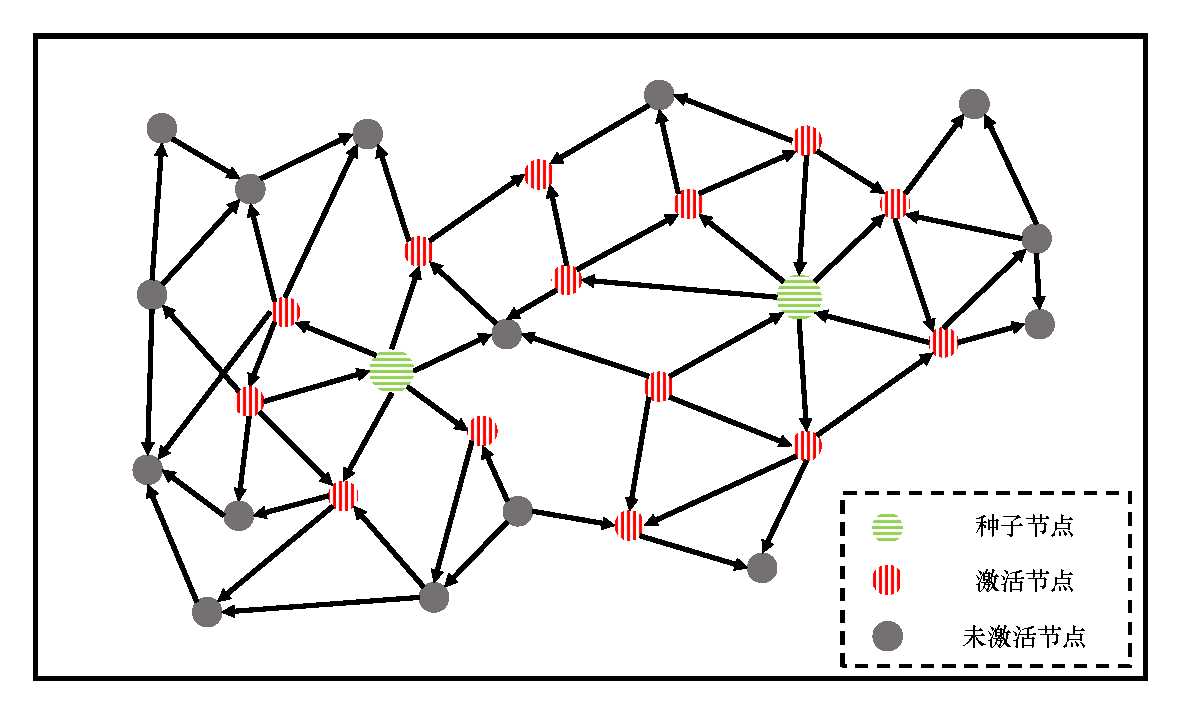
\includegraphics[width=0.8\textwidth]{infoDiffExp}
    \caption{信息传播以及影响力最大化示意图}
    \label{fig:infoDiffExp}
\end{figure}

图\ref{fig:infoDiffExp}为一个信息传播以及影响力最大化示意图,其中的点代表着个体,边代表着社交关系。图中所示的例子为选中了绿色节点为种子节点,进行信息传播后最终产生的传播范围。红色的节点代表接受了信息,灰色的节点代表未接受信息。影响力最大化的问题即是研究如何选取初始的种子节点集合,使得传播范围最大化。

市场营销是研究信息传播模型以及机理的一个典型驱动。市场营销的过程可以简述如下,一个公司希望在社交网络中通过“口碑效应”推动一款新产品或者一种新理念。一种有成本效益的方法是寻找到整个网络中有影响力的个人,然后投入资源来使他们接受这款产品,例如赠送样品、免费试用、优惠折扣等。这样的举措是希望这些有影响力的个人在接受新产品或者新理念后,能够驱使社交网络中的其他个人也来接受新产品或者新理念,然后在社交网络中产生一个大的级联效应,从而使得更多的个体接受新产品或者新理念。为了达到市场营销这一目的,我们需要对两个重要的问题进行研究:(1)如何对网络中的信息传播过程进行建模,包括模型参数的学习等;(2)如何在给定的传播模型的条件下,设计一个有效的方法来寻找能够最大化影响力的节点集合。本章着重对第二个问题进行研究。

影响力最大化问题作为市场营销的一种算法技术首先被Domingos和Richardson\upcite{domingos2001mining}所提出,该问题基于马尔科夫随机场的概率框架。而后,Kempe等人\upcite{kempe2003maximizing}首次将影响力最大化问题形式化成为一个离散的随机优化问题。信息传播的过程可以简述如下,在一个给定的网络中,选择部分节点做为种子集合,这些种子节点将会按照一定的规则去激活它们的邻居节点。被激活的节点在下一时刻将拥有能力去激活它们的邻居节点,这个过程将一直持续到没有新的节点可以被激活,整个信息传播的过程才会停止。影响力最大化问题是在给定网络和传播模型的条件下,研究如何选择种子节点集合使得传播的影响范围最大化,即激活的节点数目最大化。从上述信息传播过程的描述中,我们可以得知,一个被激活的节点会在被激活的下一时刻尝试激活它的邻居节点。因此,除去种子节点外,网络中的节点在被激活前都会有一个时间延迟,我们称之为传播时延。如果一个节点在信息传播结束时,仍然未被激活,则该节点的传播时延可以看作无穷大。而影响力最大化问题仅仅考虑了传播范围,忽略了节点的传播时延。在真实的场景中,例如市场营销、商业活动、竞选活动等,传播时延在信息传播中是一个非常重要的因素。为了让其他人接受自己的新产品或者新理念,人们总是希望能够尽快地将消息传播到群体中。我们以传播效率(\textit{influence efficiency})来表示传播时延的倒数,传播时延小,则传播效率大。如果节点在信息传播结束时仍然未被激活,那么该节点的传播效率则为0。以上是针对单个节点的传播时延和传播效率的分析,下面我们对整个网络的传播时延和传播效率进行分析。在给定一个传播网络和初始的种子节点集合的情况下,如果整个网络中所有节点的传播效率高,这就意味着在信息传播过程中,网络中的节点将被迅速地激活。我们设想如下,针对传统的影响力最大化问题有两种选择种子节点集合的策略,它们有着相同的传播范围,即能够在信息传播过程结束时能够激活相同的节点数目。但是,这两种策略中,网络中的传播时延可能是不同的,即不同策略在同一网络中的传播效率是不同的,而这一问题在传统的影响力最大化问题中是没有讨论的。

\section{相关定义}
\label{sec4:definition}
在本节中,第\ref{subsec4:model}节首先对独立级联模型(Independent Cascade Model)以及在独立级联模型下的影响力最大化问题进行回顾,然后介绍了几种解决影响力最大化问题的方法,并且对这些算法进行分析,包括影响力函数期望的单调性和子模性等。其次,第\ref{subsec4:efficiency}节提出了传播效率最大化(Influence Efficiency Maximization)问题,该问题是基于传统的影响力最大化问题,将传播时延考虑在内,研究如何使得整个网络的传播效率最大化。同时,第\ref{subsec4:efficiency}节对传播效率最大化问题进行了形式化的描述,分析了传播效率最大化和影响力最大化问题的区别。

为了便于参照,表\ref{tab:notation}中列出了频繁使用的符号。

\begin{table}[ht]
\centering
\caption{常用符号列表}
\begin{tabular}{|p{2cm}|p{10cm}|}
\hline
\textbf{符号} & \textbf{描述} \\
\hline
$\mathcal{G}=\left(\mathcal{V},\mathcal{E}\right)$ & $\mathcal{G}$是社交网络构成的图,$\mathcal{V}$是节点集合,$\mathcal{E}$是边的集合\\
\hline
$\mathcal{H}=\left(\mathcal{V},\mathcal{Z}\right)$ & $\mathcal{H}$是基于图$\mathcal{G}$生成的超图(参见算法\ref{alg:res}),$\mathcal{V}$是节点集合,$\mathcal{Z}$是超边集合\\
\hline
$n$ & $\mathcal{G}$或者$\mathcal{H}$的节点的数目 \\
\hline
$m$ & $\mathcal{G}$的边的数目 \\
\hline
$k$ & 种子节点集合的大小 \\
\hline
$p^\mathcal{G}_{u,v}$ & 节点$u$激活节点$v$的概率 \\
\hline
$I\left(S\right)$ & 种子节点集合$S$的影响力 \\
\hline
$RR\left(v\right)$ & 节点$v$的反向可达集合 (参见定义\ref{def:rrSet}) \\
\hline
$e_{u,v}$ & 节点$u$到节点$v$的传播效率(参见公式(\ref{eq:efficiency})) \\
\hline
$T\left(S\right)$ & 种子节点集合$S$在图$\mathcal{G}$中的传播效率(参见公式(\ref{eq:influenceEfficiency}))\\
\hline
$T'\left(S\right)$ & 种子节点集合$S$在超图$\mathcal{H}$中的传播效率(参见算法\ref{alg:res})\\
\hline
\end{tabular}
\label{tab:notation}
\end{table}

\subsection{传播模型以及影响力最大化问题}
\label{subsec4:model}
本章采用一种广泛采用的信息传播模型,独立级联模型,进行传播影响的研究。在该模型下,一个社交网络可被建模表示为一个有向图$\mathcal{G}=\left(\mathcal{V},\mathcal{E}\right)$,其中$\mathcal{V}$代表网络中的个体,$\mathcal{E}$表示个体之间的社会关系。此外,图中的每一条边$e_{u,v} \in \mathcal{E}$上都关联着一个传播概率$p^\mathcal{G}_{u,v}$,表示着节点$u$到节点$v$的影响力度。如果传播概率$p^\mathcal{G}_{u,v}$越大,则节点$u$更加可能激活节点$v$。如果图$\mathcal{G}$与上下文无关,本章则用$p_{u,v}$来表示节点$u$到节点$v$的传播概率。

独立级联模型描述了一个直观的信息传播过程,其过程如下。在独立级联模型下,网络中的个体会被其邻居所影响,这些影响之间是独立的。给定一个种子节点集合$S \subseteq \mathcal{V}$,信息传播在独立级联模型下是如下进行的。定义$S_t$为在$t \geq 0$的时刻,已经被激活的节点集合。显然,在$t=0$时刻时,满足$S_0=S$。在$t$时刻,每一个在$t-1$时刻被激活的节点$u \in N^{in}\left(v\right) \cap \left(S_{t-1} \setminus S_{t-2} \right)$会独立地去尝试激活它的出度边指向的未被激活的邻居节点$v \in \mathcal{V} \setminus S_{t-1}$,激活节点$v$的概率等于$p_{u,v}$。当节点$u$尝试了去激活所有它的出度边指向的节点后,它在随后的时刻不会再次尝试激活其出度邻居节点,即在$t-1$时刻被激活的节点$u$只会在$t$时刻去尝试激活它的出度边指向的邻居节点。当$t$满足$S_t = S_{t-1}$时,整个信息传播过程停止。

\begin{figure}[ht]
   \begin{minipage}{0.48\textwidth}
     \centering
     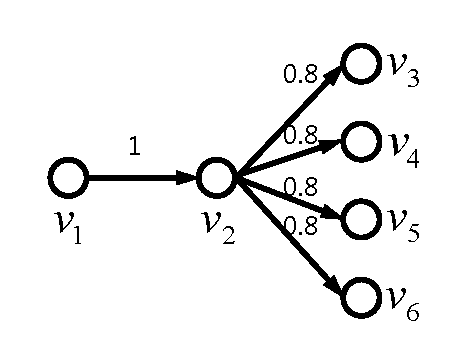
\includegraphics[width=0.8\linewidth]{tinyGraph}
     \caption{社交网络中的信息传播概率图$\mathcal{G}$}
     \label{fig:tinyGraph}
   \end{minipage}
   \hfill
   \begin {minipage}{0.48\textwidth}
     \centering
     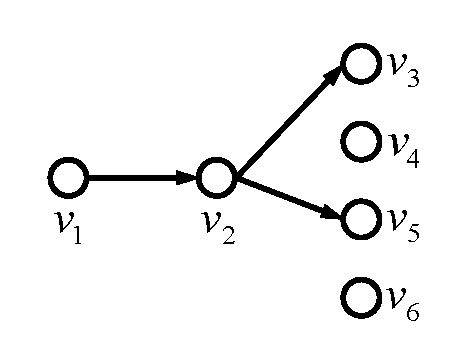
\includegraphics[width=0.8\linewidth]{tinyRandomGraph}
     \caption{随机实例图$g$}
     \label{fig:tinyRandomGraph}
   \end{minipage}
\end{figure}

以图\ref{fig:tinyGraph}中的社交网络$\mathcal{G}$为例,考虑种子节点集合$S=\left\{v_1\right\}$的信息传播过程。图\ref{fig:tinyGraph}中边上的数值代表着节点之间的传播概率$p^\mathcal{G}_{u,v}$。整个信息传播的过程可以描述如下。在$t=0$时刻,由于节点$v_1$是种子节点集合中唯一的节点,因此节点$v_1$被激活。在$t=1$时刻,因为节点$v_1$在$t=0$时刻被激活,而且图$\mathcal{G}$中存在一条从$v_1$到$v_2$概率为1的边,节点$v_1$将依概率1去激活节点$v_2$。因此,节点$v_2$将在$t=1$时刻被激活,$S_1=\left\{v_1, v_2\right\}$。此后,在$t=2$时刻,节点$v_2$将尝试去激活节点$v_3$、$v_4$、$v_5$以及$v_6$。假设这一次信息传播过程如图\ref{fig:tinyRandomGraph}所示,节点$v_3$和$v_5$被激活,则$S_2=\left\{v_1, v_2, v_3, v_5\right\}$。然后,在$t=3$时刻,由于被激活的节点没有后继节点可被激活,整个信息传播过程在此时刻停止。定义$I\left(S\right)$为在种子节点集合是$S$的条件下,整个信息传播过程中激活的节点数目,代表信息传播过程中的影响力。在上述的图$\mathcal{G}$的一次信息传播过程中,影响力$I\left(S\right)=4$。

给定一个种子节点集合$S$,定义$\mathbb{E}_\mathcal{G}\left[I\left(S\right)\right]$表示种子节点集合在图$\mathcal{G}$中影响力的期望,它等于以种子节点集合为传播源,在图$\mathcal{G}$中信息传播结束时激活节点数目的期望值。在独立级联模型下,影响力最大化问题的目标是寻找一个大小至多为$k$的种子节点集合,使得影响力函数的期望值$\mathbb{E}_\mathcal{G}\left[I\left(S\right)\right]$最大化。给定一个输入$k$,影响力最大化问题可以形式化为如第\ref{subsec1:influenceMax}小节中公式(\ref{eq:imProblem})所示。

以图\ref{fig:tinyGraph}的社交网络$\mathcal{G}$为例,给定输入$k=1$来考虑影响力最大化问题。为了解决例子中的影响力最大化问题,根据公式(\ref{eq:imProblem})所示,我们需要计算所有$k=1$的种子节点集合的影响力期望值,即每个节点的影响力期望值。对于节点$v_1$组成的种子节点集合,其影响力期望值$\mathbb{E}_\mathcal{G}\left[I\left(\{v_1\}\right)\right]=1+1+4\times0.8=5.2$。对于种子节点集合$\{v_2\}$,影响力期望值$\mathbb{E}_\mathcal{G}\left[I\left(\{v_2\}\right)\right]=1+4\times0.8=4.2$。对于其他的种子节点集合,$\mathbb{E}_\mathcal{G}\left[I\left(\{v_3\}\right)\right]=
\mathbb{E}_\mathcal{G}\left[I\left(\{v_4\}\right)\right]=
\mathbb{E}_\mathcal{G}\left[I\left(\{v_5\}\right)\right]=
\mathbb{E}_\mathcal{G}\left[I\left(\{v_6\}\right)\right]=1$。由此,我们可以得出,在给定图$\mathcal{G}$以及$k=1$的条件下,影响力最大化问题的最优解为$S^\ast=\left\{v_1\right\}$。

在上述的例子中,因为图$\mathcal{G}$的结构简单,并且种子节点集合的大小$k=1$,所以能够直接计算得出种子节点集合的影响力期望值,从而选择得出最优解。而在实际情况下,图$\mathcal{G}$的结构往往会复杂得多,而且$k>1$,很难直接计算种子节点集合的影响力期望值。Kempe等人\upcite{kempe2003maximizing}首先证明了在独立级联模型下,影响力最大化问题是一个NP-难问题。因此,直接计算出有影响力的节点是十分困难的。为了解决此问题,Kempe等人又证明了在独立级联模型下,影响力函数的期望$\mathbb{E}_\mathcal{G}\left[I\left(S\right)\right]$是单调的以及子模性的。这两个性质为求解影响力最大化问题的近似算法提供了理论保证。形式上,一个单调的函数对于任意的节点$u$和任意集合$S$,都满足$f\left(S\cup\left\{u\right\}\right) \geq f\left(S\right)$。而一个子模的函数对于任意的节点$u$以及任意的两个集合$S \subseteq W$,都满足$f\left(S\cup\left\{u\right\}\right) - f\left(S\right) \geq f\left(W\cup\left\{u\right\}\right) - f\left(W\right)$。针对具有单调性以及子模性的函数,Nemhauser等人\upcite{nemhauser1978analysis}提出了一种朴素的贪心算法来解决此类问题。算法的核心思想是首先从一个空的种子节点集合$S=\emptyset$开始,重复地选择当前边际收益(即$f\left(S\cup\left\{u\right\}\right) - f\left(S\right)$)最大的节点$u$加入到种子节点集合$S$中,直到满足种子节点集合的大小为$k$时结束迭代。选择节点$u$的准则可以形式化如下,
\begin{equation}
\label{eq:greedyIM}
    u=\arg\max\limits_{w \in V \setminus S}\left({\mathbb{E}_\mathcal{G}\left[I\left(S\cup w\right)\right]-\mathbb{E}_\mathcal{G}\left[I\left(S\right)\right]}\right)
\end{equation}

Nemhauser等人证明了朴素的贪心算法得出解以$1-1/\mathsf{e}$的因子近似于最优解,即任意一个由贪心算法的出来的解$S$都满足$I\left(S\right) \geq (1-1/\mathsf{e}) I\left(S^{\ast}\right)$,其中$S^{\ast}$代表最优解,$\mathsf{e}$为自然对数的底。虽然贪心算法的核心思想比较简单,但是由于计算影响力期望值的过程是\#P-难\upcite{chen2010scalable}的问题,因此实现该算法并不是简单的。为了解决该问题,Kempe等人\upcite{kempe2003maximizing}提出了使用蒙特卡罗(Monte Carlo)方法来对$\mathbb{E}_\mathcal{G}\left[I\left(S\right)\right]$在一定精度内进行估计。蒙特卡罗方法的步骤如下。假设我们对图$\mathcal{G}=\left(\mathcal{V},\mathcal{E}\right)$中的所有的边$e\in\mathcal{E}$都进行抛硬币实验,图$\mathcal{G}$中边的连接的概率为$p\left(e\right)$,我们以$1-p\left(e\right)$的概率移除掉边$e$。定义$g$为得到的结果图,$R_g\left(S\right)$为在图$g$中从种子节点集合$S$出发可达的节点集合。我们需要注意的是,图$g$中的边不再是概率性连接的边,而是确定性的边。对于任意节点$v\in g$,如果在图$g$中存在一条路径从节点集合$S$出发到达节点$v$,那么称节点$v$是从节点集合$S$可达的。Kempe等人\upcite{kempe2003maximizing}证明了$R_g\left(S\right)$的期望值与$\mathbb{E}_\mathcal{G}\left[I\left(S\right)\right]$是相等的,即可表示为如下,
\begin{equation}
\label{eq:influenceSpread}
    \mathbb{E}_\mathcal{G}\left[I\left(S\right)\right] = \mathbb{E}_{g\sim\mathcal{G}}\left[I_g\left(S\right)\right]
\end{equation}
其中$I_g\left(S\right) = \left\vert{R_g\left(S\right)}\right\vert$,即在图$g$中的影响力等于从种子节点集合出发可达的节点数目。因此,我们可以通过估计$R_g\left(S\right)$的期望值来估计$\mathbb{E}_\mathcal{G}\left[I\left(S\right)\right]$,即通过估计图$g$中可达的节点数目的期望来估计原图$\mathcal{G}$中的影响力期望值。在实际操作中,我们首先根据原来的社交网络生成多个实例$g\sim\mathcal{G}$,然后对每一个实例进行计算其影响力$I_g\left(S\right)$,最终计算其平均值作为$\mathbb{E}_\mathcal{G}\left[I\left(S\right)\right]$的一个估计。假设我们在估计$\mathbb{E}_\mathcal{G}\left[I\left(S\right)\right]$的过程中生成了$r$个实例图$g$,并且$r$足够大,那么在独立级联模型下,贪心算法能够得到一个$\left(1-1/\mathsf{e}-\varepsilon\right)$的近似最优解,其中$\varepsilon$是一个与图$\mathcal{G}$和$r$相关的常数\upcite{borgs2014maximizing,kempe2005influential}。一般来说,Kempe等人建议设置$r=10,000$,许多其他的工作都采用了相似的设置参数。

尽管朴素的贪心算法是有效的,但是在复杂网络的应用中,算法的效率是极其低的。算法的时间复杂度为$O\left(knmr\right)$。确切来说,算法进行了$k$次迭代来选择种子节点集合,每一次迭代需要对$O\left(n\right)$个节点进行影响力的期望值的估计。每一次估计需要对生成的$r$个实例进行计算,而每一次计算需要消耗$O\left(m\right)$的时间。因此,整个计算过程的时间复杂度为$O\left(knmr\right)$。

对于具有子模性的函数,惰性计算(\textit{lazy evaluations})技术是一种比较知名的优化方法,它能够大大的降低计算的次数,而不改变贪心算法的输出。这个技术首先由Minoux\upcite{minoux1978accelerated}作为一种加速的贪心算法提出,Leskovec\upcite{leskovec2007cost}等人通过实验验证了惰性计算针对影响力最大化问题能够加速近700倍。

即使惰性计算能够提高计算的性能,但是贪心算法仍然在效率上是不足的。究其原因,贪心算法的弊端主要是在于计算影响力期望值的过程中,它需要对$O\left(kn\right)$个节点进行估计。然而,其中大多数估计都是无用的,因为我们只关心影响力期望值最大的节点。在朴素贪心算法的框架下,这些无用的计算又是不可避免的。

为了解决朴素贪心算法的这一弊端,Borgs等人\upcite{borgs2014maximizing}提出了一种新的方法,突破了朴素贪心算法的限制。Tang等人\upcite{tang2014influence}将这种方法称之为反向传播采样(Reverse Influence Sampling),并且阐述了其工作原理。为了解释反向传播采样算法的工作原理,我们首先引入如下的概念。

\begin{defn}[反向可达集合]
\label{def:rrSet}
给定一个图$\mathcal{G}=\left(\mathcal{V}, \mathcal{E}\right)$,我们对图中的$\mathcal{G}$中的每一条边$e \in \mathcal{E}$进行抛硬币实验,依概率$1-p\left(e\right)$移除掉边$e$。定义$g$为得到的图,对于任意的节点$v \in \mathcal{V}$,节点$v$在图$g$中的反向可达集合${RR}\left(v\right)$定义为图$g$中可达节点$v$的节点集合。这就是说,如果节点$u \in {RR}\left(v\right)$,则至少在图$g$中存在一条路经从节点$u$到达节点$v$。
\end{defn}

根据定义\ref{def:rrSet}可知,如果节点$u$在节点$v$的反向可达集合${RR}\left(v\right)$中,那么节点$u$在图$\mathcal{G}$中能够依一定概率通过一条路径到达节点$v$。这也就表示,如果采用节点$u$作为种子节点集合$S=\{u\}$在图$\mathcal{G}$中进行信息传播,那么节点$u$是有一定概率激活节点$v$的。此外,Borgs等人给出了反向可达集合的性质如下,

\begin{lemma}
\label{lem:rrSet}
如果一个节点$v$的反向可达集合${RR}\left(v\right)$有$\rho$的概率与节点集合$S$存在交集,那么如果以$S$为种子节点集合在图$\mathcal{G}$中进行信息传播,则节点$v$将依概率$\rho$被激活。
\end{lemma}

\begin{proof}
假定$g$为基于$\mathcal{G}$依概率$1-p\left(e\right)$移除每一条边$e \in \mathcal{E}$生成的实例图。定义$\rho_2$为节点集合$S$在图$g$中可达节点$v$的概率,$\rho_1$为图$g$中存在一条从节点集合$S$到达节点$v$的概率。那么,根据定义\ref{def:rrSet}可知,$\rho_1 = \rho_2$。
\end{proof}

基于以上的理论,反向传播采样方法的算法流程按照如下的两步进行。第一步,首先在图$\mathcal{G}$中等概率地任意选择一个节点$v \in \mathcal{V}$,按照定义\ref{def:rrSet}来生成反向可达集合${RR}\left(v\right)$。然后,重复上述的过程来生成多个实例。第二步,选择$k$个节点来覆盖最多的反向可达集合。当且仅当一个节点$u\in RR\left(v\right)$时,我们称节点$u$覆盖集合$RR\left(v\right)$。最后,方法采用朴素贪心算法来得出一个下限为$1-1/\mathsf{e}$的近似最优解$S$作为结果返回。

反向传播采样方法的核心思想可以描述如下。如果一个节点$u$出现在许多的反向可达集合$RR\left(v\right)$中,那么节点$u$就有更高的概率去激活更多的节点。而且,节点$v$是等概率地从节点集合$\mathcal{V}$中抽取,因此节点$u$将有概率激活图$\mathcal{G}$中更多的节点,即影响力$I\left(\{u\}\right)$的值会更大。这也就是说,如果一个种子节点集合$S$覆盖了最多的反向可达集合$RR\left(v\right)$,那么$S$在图$\mathcal{G}$中将有最大的影响力期望值。

以图\ref{fig:tinyGraph}中的社交网络$\mathcal{G}$为例,考虑在独立级联模型以及$k=1$的条件下,反向传播采样方法的工作流程。第一步,首先反向传播采样方法将等概率地随机从图$\mathcal{G}$中选取节点$v$,然后依照概率$1-p\left(e\right)$移除每一条边$e$得到图$g$,然后计算反向可达集合$RR\left(v\right)$。假设我们选择了节点$v_3$并且得到的结果图$g$如图\ref{fig:tinyRandomGraph}所示,则我们可以计算得到${RR}_1=\left\{v_1, v_2, v_3\right\}$,其中下标表示生成的反向可达集合的序号。这是因为在图$g$中,$v_1$,$v_2$以及$v_3$是可达节点$v_3$的节点。然后,重复上述过程生成多个反向可达集合。假设这个过程中生成的其他反向可达集合为${RR}_2=\left\{v_1\right\}$,${RR}_3=\left\{v_1, v_2\right\}$, ${RR}_4=\left\{v_4\right\}$,${RR}_5=\left\{v_1, v_2, v_5\right\}$以及 ${RR}_6=\left\{v_6\right\}$。在这个情况下,我们可以得出节点$v_1$覆盖了最多的反向可达集合,因为节点$v_1$包含在集合${RR}_1$,${RR}_2$,${RR}_3$,${RR}_5$中。因此,反向传播采样方法返回$S=\left\{v_1\right\}$作为最终结果。

与朴素贪心算法对比,反向传播采样算法之所以效率更高是因为避免了在计算$O\left(kn\right)$次迭代的影响力期望值的无效计算。算法的核心关键点是以反向可达集合$RR$取代了对信息传播的迭代模拟。为了平衡反向传播采样方法的有效性和高效性,算法需要控制生成反向可达集合的数目。Borgs等人证明了,为了在独立级联模型下得到一个$\left(1-1/\mathsf{e}-\varepsilon\right)$的近似最优解,$RR$的数目至少为$\Theta\left(k\left(m+n\right)\log{n}/\varepsilon^3\right)$\upcite{borgs2014maximizing}。

\subsection{传播效率最大化问题}
\label{subsec4:efficiency}
传统的影响力最大化问题的目标是解决在给定种子节点集合大小$k$的条件下,计算得到使得影响力期望值最大的种子节点集合$S$。这个问题没有考虑信息的传播时延,给定不同的种子节点集合会使得网络中的节点在不同的时刻$t$被激活。在实际应用中,人们不仅关心传播影响范围的大小,也关注信息的传播效率。例如,在市场营销中,如何迅速地将一个新产品的信息传播给潜在用户是十分重要的。由此产生了一个新的问题,在一定条件下,我们如何能够计算出一个种子节点集合,使得网络的传播效率最大化。我们对传播效率定义如下。

\begin{defn}[传播效率]\label{def:ie}
假如存在一条路径从节点$u$到达节点$v$且路径中的每一个节点在信息传播结束时都是激活的,那么我们称这是一条从$u$到$v$的通路。网络中节点$u$到节点$v$之间可能存在多条通路。给定一个种子节点$u$,当信息传播过程结束时,对于图中的每一个节点$v \in \mathcal{V}$,如果节点$u$到节点$v$之间不存在通路,则节点$u$到节点$v$的传播效率$e_{u,v}=0$,否则节点$u$到节点$v$的传播效率形式化如下,
\begin{equation}\label{eq:efficiency}
    e_{u,v} = \frac{1}{t_{u,v}+1}
\end{equation}
其中$t_{u,v}$是从节点$u$到节点$v$的传播时延,即网络中节点$u$到节点$v$的最短通路的路径长度。对于节点$u$自身,传播时延$t_{u,u}=0$。给定种子节点集合$S$,传播效率函数$T\left(S\right)$形式化如下,
\begin{equation}\label{eq:influenceEfficiency}
    T\left(S\right)=\sum\limits_{v\in\mathcal{V}}{\frac{1}{t_{S,v}+1}}
\end{equation}
其中$t_{S,v}$是从集合$S$到节点$v$的传播时延,即网络中从集合$S$到节点$v$的最短通路的路径长度。
\end{defn}

以图\ref{fig:tinyGraph}为例,考虑种子节点集合$S=\left\{v_1\right\}$在图$\mathcal{G}$中的信息传播过程。假设信息传播过程的结果如图\ref{fig:tinyRandomGraph}所示。在$t=0$时刻,节点$v_1$作为种子节点被激活。下一时刻,$t=1$时节点$v_2$被节点$v_1$激活。然后,$t=2$时刻,节点$v_3$和节点$v_5$被激活。最后,在$t=3$时刻,没有新的节点可以被激活,信息传播过程结束。因此,传播效率$T\left(S\right)=1+\frac{1}{2}+2\times\frac{1}{3}=13/6$。

定义$\mathbb{E}_\mathcal{G}\left[T\left(S\right)\right]$为种子节点集合$S$在图$\mathcal{G}$中的传播效率的期望值。那么传播效率最大化问题是在给定种子节点集合大小$k$的情况下,计算得出使得传播效率期望值$\mathbb{E}_\mathcal{G}\left[T\left(S\right)\right]$最大化的种子节点集合$S$。给定一个输入$k$,传播效率最大化问题可以形式化如下,
\begin{equation}
\label{iem:Problem}
    \begin{split}
        &S^{\ast} = \arg\max{\mathbb{E}_\mathcal{G}\left[T\left(S\right)\right]}\\
        &s.t.~~S \subseteq \mathcal{V},\left\vert{S}\right\vert = k
    \end{split}
\end{equation}

以图\ref{fig:tinyGraph}为例,给定$k=1$以及图$\mathcal{G}$,考虑在独立级联模型下的传播效率最大化问题。我们能计算得出图$\mathcal{G}$中每一个节点的传播效率期望值。对于种子节点集合$S=\{v_1\}$的情况,$\mathbb{E}_\mathcal{G}\left[T\left(\{v_1\}\right)\right] = 1\times1 + 1\times\frac{1}{2} + 4\times0.8\times\frac{1}{3}\approx2.57$。对于$S=\{v_2\}$的情况,$\mathbb{E}_\mathcal{G}\left[T\left(\{v_2\}\right)\right] = 1\times1 + 4\times0.8\times\frac{1}{2} = 2.6$。对于其他的节点作为种子节点集合时,$\mathbb{E}_\mathcal{G}\left[T\left(\{v_3\}\right)\right] = \mathbb{E}_\mathcal{G}\left[T\left(\{v_4\}\right)\right] = \mathbb{E}_\mathcal{G}\left[T\left(\{v_5\}\right)\right] = \mathbb{E}_\mathcal{G}\left[T\left(\{v_6\}\right)\right] = 1$。因此,在图$\mathcal{G}$中,当$k=1$的情况下,传播效率最大化问题的最优解为$S^\ast = \left\{v_2\right\}$。与影响力最大化问题相比,我们可以得知,影响力期望值最大的种子节点集合不一定是传播效率期望值最大的集合。例如图\ref{fig:tinyGraph}表示的社交网络中,在$k=1$的情况下,种子节点集合$\left\{v_1\right\}$提供了最大的影响力期望值,种子节点集合$\left\{v_2\right\}$提供了最大的传播效率期望值。

为了解决传播效率最大化问题,我们依旧可以运用蒙特卡罗方法来估计$\mathbb{E}_\mathcal{G}\left[T\left(S\right)\right]$的值。假设图$g$是依概率$1-p\left(e\right)$移除图$\mathcal{G}$中的每一条边$e\in\mathcal{E}$后得到的实例图。在独立级联模型下,我们能够对传播效率的期望值估计如下,
\begin{equation}\label{eq:expectedIE}
    \mathbb{E}_\mathcal{G}\left[T\left(S\right)\right] = \mathbb{E}_{g\sim\mathcal{G}}\left[T_g\left(S\right)\right]
\end{equation}
其中$T_g\left(S\right)$为种子节点集合$g$在图$g$中的传播效率。

在第\ref{sec4:definition}节中,我们回顾了影响力最大化问题以及影响力函数的一些性质。影响力函数的单调性和子模性为问题的近似最优解算法提供了理论保证。基于该问题,本节将传播时延考虑在内,然后提出了传播效率最大化问题的定义。
\section{方法描述}
\label{sec4:method}
本节首先对传播效率最大化问题的复杂度,其次证明了近似最优解算法的保证,最后提出了反向效率采样(Reverse Efficiency Sampling)算法来解决传播效率最大化问题。

众所周知,影响力最大化问题在独立级联模型下是一个NP-难的问题。本节首先对传播效率最大化问题的复杂度进行分析。

\begin{theorem}\label{theo:npHard}
传播效率最大化问题在独立级联模型下是一个NP-难的问题。
\end{theorem}

\begin{proof}\label{pro:npHard}
考虑一个NP-完全的问题实例,子集覆盖(Set Cover)问题。问题的定义如下,给定一个集合$U=\left\{u_1, u_2, \cdots, u_n\right\}$的若干个子集$S_1, S_2, \cdots, S_m$,我们需要求解是否存在$k$个子集的并集与集合$U$相等。下面我们证明集合覆盖问题可以看作是传播效率最大化问题的一个特例。

给定任意一个集合覆盖问题的实例,可以定义一个与之相对应的二部图$\mathcal{G}$,节点数目等于$n+m$。图中的节点$i$对应于子集$S_i$,节点$j$对应于集合中的每一个元素$u_j \in U$。对于每一个节点$u_j \in S_i$,图中都有一条从节点$i$到节点$j$的边$\left(i,j\right)$,且边的传播概率为$p_{i,j}=1$。集合覆盖问题等同于判断在构造的二部图$\mathcal{G}$中,是否存在一个$k$个节点的集合$A$使得传播效率期望值$\mathbb{E}_\mathcal{G}\left[T\left(A\right)\right] \geq k+\frac{n}{2}$。因为二部图$\mathcal{G}$中边的传播概率非0即1,对应的信息传播是一个确定性的过程。初始化的$k$个种子节点等同于在集合覆盖问题中选择$k$个子集,而激活其余的$n$个节点相当于覆盖集合$U$。因此,如果存在$k$个节点的集合$A$满足$\mathbb{E}_\mathcal{G}\left[T\left(A\right)\right] \geq k+\frac{n}{2}$,则集合覆盖问题能够被解决。
\end{proof}

此外,另一个重要的问题是计算一个种子节点集合的传播效率期望值是非常耗时的,时间复杂度为$O\left(mr\right)$。给定一个种子节点集合$S$,没有一个高效的方法直接计算传播效率期望值$\mathbb{E}_\mathcal{G}\left[T\left(S\right)\right]$。本节将这个问题规约到$s$-$t$连通性问题\upcite{valiant1979complexity},证明了在独立级联模型下计算传播效率期望值是一个\#P-难的问题。

\begin{theorem}
\label{theo:sharpHard}
在独立级联模型下,给定一个种子节点集合$S$,传播效率期望值计算问题$\mathbb{E}_\mathcal{G}\left[T\left(S\right)\right]$是一个\#P-难的问题。
\end{theorem}

\begin{proof}
我们通过将这个问题规约到$s$-$t$连通性问题来证明定理。给定一个有向图$\mathcal{G}=\left( \mathcal{V}, \mathcal{E} \right)$以及两个节点$s$和$t$,$s$-$t$连通性问题是来计算图$\mathcal{G}$中能够连通节点$s$和节点$t$的子图数。定义$p^\mathcal{G}_{s,t}$为图$\mathcal{G}$中节点$s$与节点$t$连通的概率。当使得图$\mathcal{G}$的每一条边有$1/2$的概率连通,$1/2$的概率不连通时,我们可以直观地观察到,$s$-$t$连通性问题等同于求解$p^\mathcal{G}_{s,t}$。下一步,我们将$s$-$t$连通性问题归约到传播效率期望值计算问题。首先,令种子节点集合$S=\{s\}$,且图$\mathcal{G}$中的每一条边$\left(u,v\right) \in \mathcal{E}$的传播概率$p^\mathcal{G}_{u,v}=1/2$。此时,图$\mathcal{G}$中,以$S$为种子节点集合的传播效率期望值定义为$\mathbb{E}_\mathcal{G}\left[T_0\left(S\right)\right]$。下一步,我们在图$\mathcal{G}$增加一个节点$t_1$以及一条从节点$t$到节点$t_1$的边。我们称得到的新的图为$\mathcal{G}_1$,以及新增的边的传播概率为$p^{\mathcal{G}_1}_{t,t_1}=1$。在图$\mathcal{G}_1$中,以$S$为种子节点集合的传播效率期望值定义为$\mathbb{E}_\mathcal{G}\left[T_1\left(S\right)\right]$。而且我们可计算得知,$\mathbb{E}_\mathcal{G}\left[T_1\left(S\right)\right]=\mathbb{E}_\mathcal{G} \left[T_0\left(S\right)\right] + p^{\mathcal{G}_1}_{t,t_1}\cdot \sum_{i=1}^n{p^\mathcal{G}_{s,t,d=i}\cdot \frac{1}{d+1}}=\mathbb{E}_\mathcal{G} \left[T_0\left(S\right) \right] + \sum_{i=1}^n{p^\mathcal{G}_{s,t,d=i}\cdot \frac{1}{d+1}}$,其中$p^\mathcal{G}_{s,t,d=i}$表示在图$\mathcal{G}$中,从节点$s$到节点$t$且距离为$d$的概率(从$s$达到$t$经过通过$d$次传播),$n=\left\vert\mathcal{V}\right\vert$。下一步,我们继续在图$\mathcal{G}_1$中,添加节点$t_2$以及一条从$t_1$到$t_2$的边,得到新的图$\mathcal{G}_2$,且令$p^{\mathcal{G}_2}_{t_1,t_2}=1$。在图$\mathcal{G}_2$中,以$S$为种子节点集合的传播效率期望值定义为$\mathbb{E}_\mathcal{G}\left[T_2\left(S\right)\right]$。可以计算得知,$\mathbb{E}_\mathcal{G}\left[T_2\left(S\right)\right]=\mathbb{E}_\mathcal{G} \left[T_1\left(S\right)\right] + p^{\mathcal{G}_1}_{t_1,t_2}\cdot p^{\mathcal{G}_1}_{t,t_1}\cdot \sum_{i=1}^n{p^\mathcal{G}_{s,t,d=i}\cdot \frac{1}{d+2}}=\mathbb{E}_\mathcal{G} \left[T_1\left(S\right)\right] + \sum_{i=1}^n{p^\mathcal{G}_{s,t,d=i}\cdot \frac{1}{d+2}}$。我们可以重复上述步骤,得到$n$个以$S$为种子节点集合的传播效率期望值$T_1\left(S\right),\cdots,T_n\left(S\right)$。且递推公式为$\mathbb{E}_\mathcal{G}\left[T_j\left(S\right)\right]=\mathbb{E}_\mathcal{G} \left[T_{j-1}\left(S\right)\right] + \sum_{i=1}^n{p^\mathcal{G}_{s,t,d=i}\cdot \frac{1}{d+j}}$。这些传播效率期望值方程可以表示如下,
\begin{equation}\label{eq:sharpHard}
    \begin{bmatrix}
    \frac{1}{1+1} & \frac{1}{1+2} & \cdots & \frac{1}{1+n} \\
    \vdots & \vdots & \cdots & \vdots \\
    \frac{1}{i+1} & \frac{1}{i+2} & \cdots & \frac{1}{i+n} \\
    \vdots & \vdots & \ddots & \vdots \\
    \frac{1}{n+1} & \frac{1}{n+2} & \cdots & \frac{1}{n+n}
    \end{bmatrix}
    \begin{bmatrix}
    p^\mathcal{G}_{s,t,d=1}\\
    \vdots\\
    p^\mathcal{G}_{s,t,d=i}\\
    \vdots\\
    p^\mathcal{G}_{s,t,d=n}
    \end{bmatrix}
    =
    \begin{bmatrix}
    \mathbb{E}_\mathcal{G}\left[T_1\left(S\right)\right] - \mathbb{E}_\mathcal{G}\left[T_0\left(S\right)\right]\\
    \vdots\\
    \mathbb{E}_\mathcal{G}\left[T_i\left(S\right)\right] - \mathbb{E}_\mathcal{G}\left[T_{i-1}\left(S\right)\right]\\
    \vdots\\
    \mathbb{E}_\mathcal{G}\left[T_n\left(S\right)\right] - \mathbb{E}_\mathcal{G}\left[T_{n-1}\left(S\right)\right]\\
    \end{bmatrix}
\end{equation}
根据上述过程,可令$A$表示方程组(\ref{eq:sharpHard})中的矩阵,$\mathbf{x} = \left(p^\mathcal{G}_{s,t,d=1},p^\mathcal{G}_{s,t,d=2},\cdots,p^\mathcal{G}_{s,t,d=n}\right)^T$,$\mathbf{b}=\left(\mathbb{E}_\mathcal{G} \left[T_1\left(S\right)\right] - \mathbb{E}_\mathcal{G}\left[T_0\left(S\right)\right],\cdots,\mathbb{E}_\mathcal{G}\left[T_n\left(S\right)\right] - \mathbb{E}_\mathcal{G}\left[T_{n-1}\left(S\right)\right]\right)^T$。方程组(\ref{eq:sharpHard})可表示为$A\mathbf{x}=\mathbf{b}$。根据引理\ref{lem:nonsingular}可知矩阵$A$是一个非奇异的矩阵,因此线性方程组(\ref{eq:sharpHard})可以通过高斯-赛德尔方法在多项式时间内解决,而且构造这一个线性方程组是在线性时间内可完成的。我们可以直观地计算出图$\mathcal{G}$中节点$s$到$t$的连通概率$p^\mathcal{G}_{s,t}=\sum_{i=1}^n{p^\mathcal{G}_{s,t,d=i}}$,这也就是说节点$s$到节点$t$的概率在线性时间内可以计算。因此,$s$-$t$连通性问题是可解决的。而我们已知$s$-$t$连通性问题是一个\#P-完全的问题。因此,计算传播效率期望值是一个\#P-难的问题。
\end{proof}

定理\ref{theo:sharpHard}证明中的矩阵$A$如公式(\ref{eq:matrixA})所示,
\begin{equation}
\label{eq:matrixA}
	A = 
    \begin{bmatrix}
    \frac{1}{1+1} & \frac{1}{1+2} & \cdots & \frac{1}{1+n} \\
    \vdots & \vdots & \cdots & \vdots \\
    \frac{1}{i+1} & \frac{1}{i+2} & \cdots & \frac{1}{i+n} \\
    \vdots & \vdots & \ddots & \vdots \\
    \frac{1}{n+1} & \frac{1}{n+2} & \cdots & \frac{1}{n+n}
    \end{bmatrix}
\end{equation}

上述过程将计算传播效率期望值$\mathbb{E}_\mathcal{G}\left[T\left(S\right)\right]$的问题规约到了$s$-$t$连通性问题,证明了计算传播效率期望值$\mathbb{E}_\mathcal{G}\left[T\left(S\right)\right]$的问题是一个\#P-难的问题。其中引用了矩阵$A$为非奇异矩阵的事实,下面我们证明上述的矩阵$A$是非奇异的。首先,我们可以观察到矩阵$A$是一个对称矩阵,其次我们可以得到矩阵中通项$a_{ij}$。因此,我们考虑使用行列变换对矩阵$A$的行列式进行降维,发现行列式的递推公式,计算行列式的值。如果行列式不为零,则可证明矩阵$A$是非奇异的。引理以及其详细证明过程如下。

\begin{lemma}\label{lem:nonsingular}
矩阵$A \in \mathbb{R}^{n \times n}$且$a_{ij} = \frac{1}{i+j}$,则矩阵$A$是非奇异的。
\end{lemma}
\begin{proof}
令$\Delta_{n}$表示矩阵$A$的行列式,
\begin{equation}\label{eq:detetminant1}
    \Delta_{n}=\left\vert A \right\vert=
    \begin{vmatrix}
    \frac{1}{1+1} & \frac{1}{1+2} & \cdots & \frac{1}{1+n} \\
    \vdots & \vdots & \cdots & \vdots \\
    \frac{1}{i+1} & \frac{1}{i+2} & \cdots & \frac{1}{i+n} \\
    \vdots & \vdots & \ddots & \vdots \\
    \frac{1}{n+1} & \frac{1}{n+2} & \cdots & \frac{1}{n+n}
    \end{vmatrix}
\end{equation}
下一步,令行列式$\left\vert A \right\vert$中的第$i$行($2\leq i \leq n$)减去第1行,可得到$a_{ij} = \frac{1}{i+j}-\frac{1}{1+j}=\frac{1-i}{\left(i+j\right)\left(1+j\right)}$。则行列式$\Delta_n$可表示为如下所示。
\begin{equation}\label{eq:detetminant2}
\begin{split}
    \Delta_n & =
    \begin{vmatrix}
    \frac{1}{1+1} & \frac{1}{1+2} & \cdots & \frac{1}{1+n} \\
    \vdots & \vdots & \cdots & \vdots \\
    \frac{1-i}{\left(i+1\right)\left(1+1\right)} & \frac{1-i}{\left(i+2\right)\left(1+2\right)} & \cdots & \frac{1-i}{\left(i+n\right)\left(1+n\right)} \\
    \vdots & \vdots & \ddots & \vdots \\
    \frac{1-n}{\left(n+1\right)\left(1+1\right)} & \frac{1-n}{\left(n+2\right)\left(1+2\right)} & \cdots & \frac{1-n}{\left(n+n\right)\left(1+n\right)} \\
    \end{vmatrix}\\
    & =
    \frac{\prod\limits_{2\leq i \leq n}{1-i}}{\prod\limits_{1\leq j \leq n}{1+j}}
    \begin{vmatrix}
    1 & 1 & \cdots & 1 \\
    \frac{1}{2+1} & \frac{1}{2+2} & \cdots & \frac{1}{2+n} \\
    \vdots & \vdots & \cdots & \vdots \\
    \frac{1}{i+1} & \frac{1}{i+2} & \cdots & \frac{1}{i+n} \\
    \vdots & \vdots & \ddots & \vdots \\
    \frac{1}{n+1} & \frac{1}{n+2} & \cdots & \frac{1}{n+n}
    \end{vmatrix}\\
    & = \frac{\prod\limits_{2\leq i \leq n}{1-i}}{\prod\limits_{1\leq j \leq n}{1+j}}
    \left\vert B \right\vert
\end{split}
\end{equation}
下一步,令行列式$\left\vert B \right\vert$中的第$j$列($2 \leq j \leq n$)减去第1列,可得$b_{ij} = \frac{1}{i+j} - \frac{1}{i+1}=\frac{1-j}{\left(i+j\right)\left(i+1\right)}$。则行列式$\Delta_n$可表示为如下所示。
\begin{equation}\label{eq:detetminant3}
\begin{split}
    \Delta_n & = \frac{\prod\limits_{2\leq i \leq n}{1-i}}{\prod\limits_{1\leq j \leq n}{1+j}}
    \begin{vmatrix}
    1 & 0 & \cdots & 0 \\
    \frac{1}{2+1} & \frac{1-2}{\left(2+2\right)\left(2+1\right)} & \cdots & \frac{1-n}{\left(2+n\right)\left(2+1\right)} \\
    \vdots & \vdots & \cdots & \vdots \\
    \frac{1}{i+1} & \frac{1-2}{\left(i+2\right)\left(i+1\right)} & \cdots & \frac{1-n}{\left(i+n\right)\left(i+1\right)} \\
    \vdots & \vdots & \ddots & \vdots \\
    \frac{1}{n+1} & \frac{1-2}{\left(n+2\right)\left(n+1\right)} & \cdots & \frac{1-n}{\left(n+n\right)\left(n+1\right)}
    \end{vmatrix}\\
    & = \frac{\prod\limits_{2\leq i \leq n}{1-i}\prod\limits_{2\leq j \leq n}{1-j}}{\prod\limits_{1\leq j \leq n}{1+j}\prod\limits_{2\leq i \leq n}{1+i}}
    \begin{vmatrix}
    1 & 0 & \cdots & 0 \\
    \frac{1}{2+1} & \frac{1}{2+2} & \cdots & \frac{1}{2+n}\\
    \vdots & \vdots & \cdots & \vdots \\
    \frac{1}{i+1} & \frac{1}{i+2} & \cdots & \frac{1}{i+n}\\
    \vdots & \vdots & \ddots & \vdots \\
    \frac{1}{n+1} & \frac{1}{n+2} & \cdots & \frac{1}{n+n}
    \end{vmatrix}\\
    & = \frac{\prod\limits_{2\leq i \leq n}{1-i}\prod\limits_{2\leq j \leq n}{1-j}}{\prod\limits_{1\leq j \leq n}{1+j}\prod\limits_{2\leq i \leq n}{1+i}}
    \begin{vmatrix}
    \frac{1}{2+2} & \frac{1}{2+3} & \cdots & \frac{1}{2+n}\\
    \vdots & \vdots & \cdots & \vdots \\
    \frac{1}{i+2} & \frac{1}{i+3} & \cdots & \frac{1}{i+n}\\
    \vdots & \vdots & \ddots & \vdots \\
    \frac{1}{n+2} & \frac{1}{n+3} & \cdots & \frac{1}{n+n}
    \end{vmatrix}\\ 
    &= \lambda_{n} \Delta_{n-1}
\end{split}
\end{equation}
其中$\lambda_{n}$是非零的。因此,我们可以重复上述步骤,则行列式$\Delta_n$可计算得到如下。
\begin{equation}\label{eq:detetminant4}
\begin{split}
    \Delta_n &= \prod\limits_{k=1}^{n-1}{\lambda_k}\Delta_1=\prod\limits_{k=1}^{n-1}{\frac{\prod\limits_{k+1 \leq i \leq n}{k-i}\prod\limits_{k+1 \leq j \leq n}{k-j}}{\prod\limits_{k \leq j \leq n}{k+j}\prod\limits_{k+1 \leq i \leq n}{k+i}}}\Delta_1\\
    & = \frac{1}{2n}\frac{\prod\limits_{2\leq k+1\leq i \leq n}{k-i}\prod\limits_{2\leq k+1\leq j \leq n}{k-j}}{\prod\limits_{1\leq k\leq j \leq n}{k+j}\prod\limits_{2\leq k+1\leq i \leq n}{k+i}}
\end{split}
\end{equation}
由上述可知$\Delta_n$中的每一项都不为零,所以可知$\Delta_n \neq 0$,因此$A$是非奇异的。
\end{proof}

由此可知,直接来求解传播效率最大化问题是非常困难的。针对这种情况,Nemhauser等人\upcite{nemhauser1978analysis}证明了一个非负的,单调的且子模性的函数$f(\cdot)$,朴素的贪心算法能够提供一个$(1-1/\textsf{e})$的近似最优解。在独立级联模型模型下的传播效率最大化问题的近似最优解的保证可以表示如下,
\begin{theorem}\label{theo:submodular}
对于在独立级联模型下的一个网络$\mathcal{G}$的任意一个实例,传播效率函数的期望$\mathbb{E}_\mathcal{G}\left[T\left(\cdot\right)\right]$是具有子模性的。
\end{theorem}

$\mathbb{E}_\mathcal{G}\left[T\left(\cdot\right)\right]$的单调性是显而易见的,因为向任意一个种子节点集合$S$中增加一个节点$u$不会使得传播效率减小。这也就是说,对于任意的种子节点集合$S$与节点$u \in \mathcal{V}$,$\mathbb{E}_\mathcal{G}\left[T\left( S \cup \left\{u\right\} \right)\right] \geq \mathbb{E}_\mathcal{G}\left[T\left(S\right)\right]$始终是成立的。为了证明定理\ref{theo:submodular}的结论,我们需要计算$\mathbb{E}_\mathcal{G}\left[T\left( S \cup \left\{u\right\} \right)\right] - \mathbb{E}_\mathcal{G}\left[T\left(S\right)\right]$的值,即我们需要计算将节点$u$加入到集合$S$中的边际收益。但是直接计算边际收益是十分困难的,因为整个信息传播过程是不确定的,节点被激活的顺序也是不确定的。为了解决这个难点,我们采用另一种等同的视角\upcite{kempe2003maximizing}来看待信息传播过程,它与节点激活的顺序无关。它提供了一种另外的途径来证明$\mathbb{E}_\mathcal{G}\left[T\left(\cdot\right)\right]$的子模性。考虑如下情景,在独立级联模型下的信息传播过程中,当节点$u$在上一时刻被激活,尝试依概率$p_{u,v}$去激活它的出度边指向的邻居节点$v$。我们可以对该过程用抛一枚偏置为$p_{u,v}$的硬币的结果来模拟,我们直观上地可以知道抛硬币实验在当节点$u$被激活后进行还是在信息传播过程的一开始就进行,然后在节点$u$被激活后再揭晓结果,这个对于模拟是不影响的。因此,我们能在信息传播过程一开始,就对于图$\mathcal{G}$中的每一条边$e=\left(u,v\right)$进行偏置为$p_{u,v}$的抛硬币实验,然后在节点$u$被激活而节点$v$没有激活的时刻揭晓结果。

令所有的抛硬币的模拟在信息传播过程的一开始就完成,则信息传播过程可以看作如下的过程。每条边$e=\left(u,v\right)$的抛硬币模拟,代表着节点$u$到节点$v$的尝试激活。如果激活成功,则我们称$e$是一条连通边。此外,我们可以称从节点$u$到节点$v$的路径是一条通路,如果路径中的每一条边都是连通边。基于上述的定义,我们可以很清晰地计算出在所有的抛硬币模拟都已确定的情况下,独立级联模型下种子节点集合为$S$的传播效率。信息传播过程结束时,当且仅当存在一条从$S$到节点$v$的通路时,节点$v$是激活的。我们可以根据从$S$到$v$的最短的通路,计算得到节点$v$的传播效率$e_{S,v}$。考虑如下一个概率空间,空间中的每一个节点代表着图$\mathcal{G}$中所有边$e$对应的抛硬币模拟的结果。令$X$表示空间中的一个样本点,且定义$T_X\left(S\right)$为以$S$为种子节点集合,抛硬币模拟结果为$X$的传播效率,$T_X\left(S\right)$可根据公式(\ref{eq:influenceEfficiency})计算得出。本节对定理\ref{theo:submodular}进行证明如下。

\begin{figure}[!ht]
    \centering
    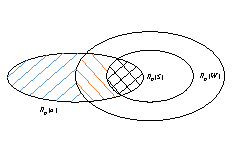
\includegraphics[width=0.8\textwidth]{submodular}
    \caption{$R_X\left(u\right)$,$R_X\left(S\right)$以及$R_X\left(W\right)$的示意图}
    \label{fig:submodular}
\end{figure}

\begin{proof}\label{pro:submodular}
首先,我们证明对于概率空间中任意的确定的样本点$X$,传播效率函数$T_X\left(\cdot\right)$是具有子模性的。为了证明上述的结论,令$S$和$W$为两个节点集合,且满足$S \subseteq W \subseteq \mathcal{V}$,令$u \in \mathcal{V}$为图$\mathcal{G}$中的任意一个节点。令$\delta\left(u|S\right)$为添加节点$u$至集合$S$后传播效率的边际收益,$\delta\left(u|S\right) = T_X\left(S\cup\left\{u\right\}\right)-T_X\left(S\right)$。然后,我们对$\delta\left(u|S\right)$和$\delta\left(u|W\right)$进行比较。为了方便比较,令$R_X\left(u\right)$表示节点$u$在样本点$X$下的可达节点集合。因为$S \subseteq W$,所以可得$R_X\left(S\right) \subseteq R_X\left(W\right)$。当节点$u$加入到集合$S$和$W$中时,会出现如图\ref{fig:submodular}三种情况。首先,第一种情况如图中的斜线区域,即对于节点$v \in R_X\left(u\right) \setminus R_X\left(W\right)$。在此种情况下,在加入节点$u$之前,图中不存在从集合$S$或者集合$W$到达节点$v$的通路。因此,可知第一种情况中$\delta\left(u|S\right) = \delta\left(u|W\right)$。第二种情况是图中的反斜线区域,即对于节点$v \in \left( R_X\left(u\right) \cap R_X\left(W\right) \right) \setminus R_X\left(S\right)$。在此种情况下,在加入节点$u$之前,图中存在从集合$W$到节点$v$的通路,但是不存在从集合$S$到节点$v$的通路。在此情况下,可知$\delta\left(u|S\right) \geq \delta\left(u|W\right)$。第三种情况是图中的网状区域,即对于节点$v \in R_X\left(u\right) \cap R_X\left(S\right)$。在此种情况下,在节点$u$前,从集合$S$或者集合$W$都有到节点$v$的通路。因为$S \subseteq W$,$e_{W,v} \geq e_{S,v}>0$,所以在第三种情况下$\delta\left(u|S\right) \geq \delta\left(u|W\right)$也是成立的。综合上述可知,结论$\delta\left(u|S\right) \geq \delta\left(u|W\right)$在任意情况下都是成立的,即$T_X\left(S\cup\left\{u\right\}\right)-T_X\left(S\right) \geq T_X\left(W\cup\left\{u\right\}\right)-T_X\left(W\right)$对于集合$S \subseteq W$是成立的,因此$T_X\left(\cdot\right)$是具有子模性的。而又有$\mathbb{E}_\mathcal{G}\left[T\left(S\right)\right] = \sum\nolimits_X{\Pr\left[X\right] \cdot T_X\left(S\right)}$,即传播效率期望值是概率空间中所有可能样本$X$的加权平均值。一个非负的线性组合不会改变函数的子模性,故传播效率函数的期望$\mathbb{E}_\mathcal{G}\left[T\left(\cdot\right)\right]$也是具有子模性。
\end{proof}

\begin{algorithm}[!ht]
\caption{$greedy(k,T)$}
\label{alg:greedy}
\begin{algorithmic}[1]
	\REQUIRE $k,\mathcal{G},T$
    \ENSURE $S$
    \STATE initialize $S=\emptyset$
    \FOR{$i$ =1 to $k$}
        \STATE select $u=\arg\max_{w \in V \setminus S}\left({\mathbb{E}_\mathcal{G}\left[T\left(S\cup w\right)\right]-\mathbb{E}_\mathcal{G}\left[T\left(S\right)\right]}\right)$
        \STATE $S=S\cup u$
    \ENDFOR
    \STATE return $S$
\end{algorithmic}
\end{algorithm}

根据定理\ref{theo:submodular}我们可知传播效率函数的期望值$\mathbb{E}_\mathcal{G}\left[T\left(\cdot\right)\right]$是单调且子模性的,因此朴素贪心算法(\textit{greedy})能够得到一个$1-1/\mathsf{e}$的近似最优解。朴素贪心算法的过程如算法\ref{alg:greedy}所示。算法的流程如下,需要求解的种子节点集合$S$首先置为空集。其次,遍历所有节点,选择传播效率期望值边际收益最大的节点$u$加入到集合$S$中。然后,重复第二步直到集合$S$的大小等于$k$。

此外,由于传播效率期望值具有子模性,因此惰性计算技术\upcite{minoux1978accelerated}可以用来提升朴素贪心算法的性能。惰性计算能够极大地减少模拟评估的次数而不改变贪心算法的的输出。正如惰性计算的名字,该方法的核心思想是尽可能地避免不必要的模拟评估。给定一个单调且子模性的函数$f$,令$f\left(u|S\right)$为集合$S$加入节点$u$后的边际收益,即$f\left(u|S\right) = f\left( S \cup \left\{u\right\} \right) - f\left( S \right)$。假设第$i$轮迭代贪心算法得出的种子节点集合为$S$,且我们对节点$u \in \mathcal{V} \setminus S$的边际收益$f\left(u|S\right)$进行了计算。在更早的迭代中,种子节点集合为$S' \subset S$,且我们计算了节点$w \in \mathcal{V} \setminus S'$的边际收益$f\left(w|S'\right)$。那么当$f\left(w|S'\right) \leq f\left(u|S\right)$时,根据子模性可知$f\left(w|S\right) \leq f\left(w|S'\right) \leq f\left(u|S\right)$。这就是说,在第$i$轮迭代中,节点$w$不可能成为最大化传播效率的节点,因此计算$f\left(w|S\right)$是没有意义的。上述的思想可以通过一个优先队列来实现,如算法\ref{alg:lazygreedy}所示,称之为惰性贪心(\textit{lazy greedy})算法。

\begin{algorithm}[!ht]
    \caption{$LazyGreedy(k,T)$}
    \label{alg:lazygreedy}
    \begin{algorithmic}[1]
	\REQUIRE $k,\mathcal{G},T$
    \ENSURE $S$
    \STATE initialize $S=\emptyset$, priority queue $Q=\emptyset$, iteration $i=1$
    \FOR{$j=1$ to $n$}
        \STATE $u.mg=T\left(u|\emptyset\right)$, $u.i=1$
        \STATE put $u$ into $Q$ with $u.mg$ as the key
    \ENDFOR
    \WHILE{$i \leq k$}
        \STATE pop the top element $u$ of $Q$
        \IF{$u.i = i$}
            \STATE $S = S \cup \left\{u\right\}$, $i=i+1$
        \ELSE
            \STATE $u.mg=T\left(u|S\right)$,  $u.i=i$ 
        \ENDIF
    \ENDWHILE
    \STATE \textbf{return} $S$
    \end{algorithmic}
\end{algorithm}

算法的具体实现过程如下。对于每一个节点$u$,我们为之设计一种结构体,包含两个域值$u.mg$以及$u.i$。其中$u.mg$表示最新一次迭代将节点$u$加入集合$S$时的传播效率期望值边际收益,$u.i$表示$u.mg$更新时的迭代轮数。初始化时,我们对所有节点$u$计算$T\left(u|\emptyset\right)$作为$u.mg$加入优先队列$Q$中,以$u.mg$作为队列的键,此时所有的$u.i=1$。此后的每一轮迭代,我们选择队列$Q$的队首(具有最大的边际收益)的节点$u$进行检查。如果$u.i=i$,即节点$u$确实是第$i$迭代时加入到种子节点集合$S$中的边际收益最大的节点,则将节点$u$加入到种子节点集合$S$中。如果$u.i \neq i$,则更新$u.mg$为$T\left(u|S\right)$,更新$u.i$为当前的迭代轮数,然后将节点$u$插入回优先队列$Q$中。

惰性贪心算法极大地减少了无效模拟评估的次数。Leskovec等人\upcite{leskovec2007cost}通过实验证明该算法对影响力最大化问题的速度提升了近700倍。对于传播效率最大化问题,由于传播效率函数的单调性和子模性,惰性贪心算法也能减少无效模拟评估次数,从而进行加速。

由定理\ref{theo:sharpHard}可知,直接计算传播效率期望值是很困难的。许多相关的工作\upcite{leskovec2007cost,goyal2011celf++,chen2009efficient}在贪心算法的框架下对此类问题进行了改进。然而,这些改进算法仍然不够高效。另一方面,启发式的算法能够解决效率问题,但是不能提供理论上的性能保证。本节借鉴了Borgs等人\upcite{borgs2014maximizing}的反向传播采样思想来解决传播效率最大化问题。

\begin{algorithm}[!ht]
    \caption{$RES$($k$,$r$,$T'\left(\cdot\right)$)}
    \label{alg:res}
    \begin{algorithmic}[1]
	\REQUIRE $k,r,T'$
    \ENSURE $S$
    \STATE {initialize $\mathcal{H}=\left(\mathcal{V}, \emptyset \right)$}
    \FOR{$i=1$ to $r$}
        \STATE{stochastically select a node $v \in \mathcal{V}$ uniformly}
        \STATE{generate $z_i = RR\left(v\right)$}
        \STATE{calculate $e_{u,v} = \frac{1}{t_{u,v}+1}$ for $u \in RR\left(v\right)$}
        \STATE{add $z_i$ to the edge set $\mathcal{Z}$ of $\mathcal{H}$}
    \ENDFOR
    \STATE{initialize $S=\emptyset$}
    \FOR{$j=1$ to $k$}
        \STATE{$w = \arg\max_{v \in \mathcal{V}}\left(T'\left(S \cup v\right) - T'\left(S\right)\right)$}
        \STATE{add $w$ to $S$}
        \STATE{remove $w$ from $\mathcal{V}$}
    \ENDFOR
    \STATE {return $S$}
    \end{algorithmic}
\end{algorithm}

如算法\ref{alg:res}所示,我们称之为反向效率采样(Reverse Efficiency Sampling),算法的流程可描述如下。反向效率采样算法按照两步进行。第一步是根据图$\mathcal{G}$建立超图$\mathcal{H}=\left(\mathcal{V}, \mathcal{Z} \right)$,其中$\mathcal{V}$是与图$\mathcal{G}$相同的节点集合,$\mathcal{Z}$是超边集合。每一条超边$z_i \in \mathcal{Z}$代表一个反向可达集合$RR\left(v\right)$,其中节点$v \in \mathcal{V}$,是随机等概率选取的。超边$z_i$可以形式化为一个集合$\{u_1, u_2, \cdots, u_j\}$,代表着存在一条从节点$u \in z_i$到节点$v$的通路。我们不断地随机等概率选取节点$v$,然后基于图$\mathcal{G}$生成图$g$,计算反向可达集合$RR\left(v\right)$,即超边$z_i$,然后添加到超边集合$\mathcal{Z}$中。该过程通过模拟图$\mathcal{G}$的反向图中的信息传播过程来实现。在反向图中首先激活节点$v$,然后按照宽度优先搜索来概率性地激活出度边指向的邻居节点。当信息传播过程停止时,被激活的节点集合构成了超图$\mathcal{H}$中的一条边。同时,我们还需要记录超边上每一个节点$u \in z_i$的传播效率$e_{u,v} = \frac{1}{t_{u,v}+1}$。我们重复生成超边的过程来构建超边集合$\mathcal{Z}$直到集合的大小到达预定的值$r$。

在第二步中,我们基于超图$\mathcal{H}$来计算种子节点集合$S$。在这一步中,算法重复地选择当前传播效率边际收益最大的节点$w \in \mathcal{V}$加入到结合$S$中,其中边际效益为$T'\left(S \cup w\right) - T'\left(S\right)$,且$T'\left(S\right) = \sum_{i=1}^r{\frac{1}{t_{S,v_i}+1}}$,$v_i$为第i轮迭代中随机等概率选取的节点,对应的超边为$z_i$。最终,算法得到一个大小为$k$的节点集合$S$。

下一步,我们对算法\ref{alg:res}进行详细地分析。首先,我们可以观察到种子节点集合$S$的传播效率期望值等于$n$倍从集合$S$到节点$u$的传播效率$e_{S,u}$,其中节点$u$从图$g$中随机等概率选取的,图$g$是基于图$\mathcal{G}$生成的实例图。上述现象可表述为如下,
\begin{theorem}\label{theo:observe}
$\mathbb{E}_{g\sim\mathcal{G}}\left[T_g\left(S\right)\right]=n\Pr\nolimits_{v,g\sim\mathcal{G}}\left[S\cap RR\left(v\right)\neq\emptyset\right]\cdot\frac{1}{d_{S,v}+1}$
\end{theorem}
\begin{proof}
    \begin{equation*}
        \begin{split}
            \mathbb{E}_{g\sim\mathcal{G}}\left[T_g\left(S\right)\right] & = \sum\limits_{v \in \mathcal{V}}{\Pr\nolimits_{g \sim \mathcal{G}}{\left[ \exists u \in S, v \in R_g \left(u\right) \right] \cdot \frac{1}{d_{S,v}+1}}}\\
            & = \sum\limits_{v \in \mathcal{V}}{\Pr\nolimits_{g \sim \mathcal{G}}{\left[ \exists u \in S, u \in {RR}_g \left(v\right) \right] \cdot \frac{1}{d_{S,v}+1}}}\\
            & = n \Pr\nolimits_{v,g \sim \mathcal{G}}{\left[ \exists u \in S, u \in {RR}_g \left(v\right) \right] \cdot \frac{1}{d_{S,v}+1}}\\
            & = n \Pr\nolimits_{v,g \sim \mathcal{G}}{\left[ S \cap {RR}_g \left(v\right) \neq \emptyset \right] \cdot \frac{1}{d_{S,v}+1}}
        \end{split}
    \end{equation*}
\end{proof}

定理\ref{theo:observe}表示我们可以通过观察事件$S\cap {RR}_g\left(v\right)\neq\emptyset$的概率来计算$\mathbb{E}_\mathcal{G}\left[T\left(S\right)\right]$。超图$\mathcal{H}$中节点$u \in \mathcal{V}$的度即为信息传播模拟过程中成功激活的节点次数。因此,由定理\ref{theo:observe}可知,我们能够基于超图$\mathcal{H}$来计算传播效率期望值。给定种子节点集合$S$与超图$\mathcal{H}$下的传播效率函数如下所示,
\begin{equation}\label{eq:infEffHyper}
    T'\left(S\right)=\sum\limits_{z_i\in\mathcal{Z}}{\frac{1}{t_{S,v_i}+1}}
\end{equation}
其中$S$为种子节点集合,$z_i$为随机等概率选取的节点$v_i$对应的超边。下一步,我们分析在超图$\mathcal{H}$中的传播效率函数期望值$\mathbb{E}_\mathcal{H}\left[T'\left(\cdot\right)\right]$。我们给出定理如下,
\begin{theorem}\label{theo:hyperSubmodular}
对于在独立级联模型下的一个网络$\mathcal{G}$的任意一个实例,对应生成的超图$\mathcal{H}$中传播效率函数的期望$\mathbb{E}_\mathcal{H}\left[T'\left(\cdot\right)\right]$是具有子模性的。
\end{theorem}
\begin{proof}
易证$\mathbb{E}_\mathcal{H}\left[T'\left(\cdot\right)\right]$是单调性的,因为将任意节点$u$加入到任意种子节点集合$S$中都不会减少传播效率期望值。为了证明子模性,我们可以先证明$T'\left(\cdot\right)$的子模性。假设种子节点集合$S$与$W$满足$S \subseteq W \subseteq \mathcal{V}$,节点$u \in \mathcal{V}$是超图$\mathcal{H}$中的节点。如果集合$S \cap z \neq \emptyset$,则我们称集合$S$覆盖超边$z$。与定理\ref{theo:submodular}相同,当将节点$u$加入集合$S$与$W$时,将有三种情况。第一种情况是集合$S$与$W$都不覆盖超边$z$,则$T'\left(S \cup u\right) - T'\left(S\right) = T'\left(W \cup u\right) - T'\left(W\right)$,即二者的边际效益相等。第二种情况是集合$S$不覆盖超边$z$,集合$W$覆盖超边$z$。此种情况下$e_{S,v} = 0$,而$e_{W,v} > 0$,故$T'\left(S \cup u\right) - T'\left(S\right) \geq T'\left(W \cup u\right) - T'\left(W\right)$。第三种情况是集合$S$与$W$都覆盖超边$z$。此种情况下由于$S \subseteq W$,所以$e_{S,v} \leq e_{W,v}$,故$T'\left(S \cup u\right) - T'\left(S\right) \geq T'\left(W \cup u\right) - T'\left(W\right)$。所以对于所有情况,我们都能得出结论$T'\left(S \cup u\right) - T'\left(S\right) \geq T'\left(W \cup u\right) - T'\left(W\right)$在独立级联模型下,$S \subseteq W$的情况下是成立的,因此$T'\left(\cdot\right)$是子模性的。而期望是对$T'\left(\cdot\right)$的加权线性求和,故$\mathbb{E}_\mathcal{H}\left[T'\left(\cdot\right)\right]$也是子模性的。
\end{proof}

由于传播效率函数期望值$\mathbb{E}_\mathcal{H}\left[T'\left(\cdot\right)\right]$是单调且子模的,则算法\ref{alg:res}中的反向效率采样算法能够得到一个$\left(1-1/\mathsf{e}-\varepsilon\right)$的近似最优解来解决独立级联模型下的传播效率最大化问题。其中$\varepsilon$与采样的次数$r$以及图$\mathcal{G}$的结构有关。如何计算$\varepsilon$与$r$以及$\mathcal{G}$的关系仍然是一个开放性的问题。下面本节对上述提及的算法的时间复杂度进行分析。其中朴素贪心算法和惰性贪心算法都是基于贪心算法框架下实现的。这一类算法进行$k$轮迭代来选择种子节点集合$S$,每一轮迭代需要对$O\left(n\right)$个节点进行传播效率期望值的估计。而每一次传播效率期望值的估计需要在$r$个生成的实例图$g$上进行$O\left(m\right)$次计算。因此,朴素贪心算法和惰性贪心算法的时间复杂度都是$O\left(knmr\right)$的。但是由于惰性贪心算法基于惰性计算避免了一些不必要的模拟评估,惰性贪心算法在实际运行中比朴素贪心算法的效率要高。相比之下,反向效率采样算法是在另一个框架下设计的。首先,反向传播采样算法生成了$r$条超边,构造了超图$\mathcal{H}$,每生成一条超边需要消耗$O\left(m\right)$的时间,因此生成整个超图$\mathcal{H}$需要消耗$O\left(rm\right)$的时间。然后,算法迭代$k$轮来生成种子节点集合$S$,每一轮迭代需要对$O\left(n\right)$个节点进行模拟估计,每一次模拟估计需要对$r$条超边进行运算,因此计算种子节点集合$S$的时间复杂度为$O\left(knr\right)$。有上述分析可知,反向效率采样的时间复杂度相比于朴素贪心算法和惰性贪心算法要低。

\section{实验分析}
\label{sec4:experiment}
本节设计了若干组实验来验证上述提出的算法。首先,我们介绍实验的设置。其次,我们详细地展示了实验结果,并对其进行分析。本节中的实验基于八核(Intel Xeon 1.80GHz CPU)、64GB内存的机器运行,操作系统为64位 CentOS release 6.7。以上所有算法都是基于Java实现,在JDK 1.8.0\_40环境下编译。
\subsection{实验设置}
\label{subsec4:settings}
本小节介绍实验的设置,包括数据集、传播模型以及算法等。
\begin{table}[!ht]
\centering
\caption{数据集特征}
\label{tab:dataset}
\begin{tabular}{ |c|c|c|c|c| }
\hline
\textbf{数据集} & \textbf{节点数} & \textbf{边数} & \textbf{类型} & \textbf{平均度} \\
\hline
\textit{Facebook} & 4k & 88k & 无向图 & 43.7\\
\hline
\textit{HepPh} & 35k & 422k & 有向图 & 24.4\\
\hline
\textit{Twitter} & 81k & 1.8M & 有向图 & 43.5\\
\hline
\textit{DBLP} & 655k & 2M & 无向图 & 6.1\\
\hline
\end{tabular}
\end{table}

在数据集方面,表\ref{tab:dataset}描述了实验所用的数据集,包括脸书(\textit{Facebook})、高能物理论文引用网络(\textit{HepPh})、推特(\textit{Twitter})、计算机科学合作网络(\textit{DBLP})。这些网络都是相关研究中使用频繁的标注数据集,可以从SNAP\upcite{snapnets}网站上下载得到。实验数据集中的网络有着不同大小的网络和特性,因此能够比较好地验证本章提出的算法。实验数据集包括两个无向图以及两个有向图。其中\textit{Facebook}与\textit{Twitter}是社交网络,如果在\textit{Facebook}网络中用户$u$与用户$v$是好友关系或者在\textit{Twitter}网络中用户用户$v$关注了用户$u$,则在对应的图中存在一条从节点$u$到节点$v$的边$e=(u,v)$。网络\textit{HepPh}为arXiv电子出版高能物理论文的引用网络。如果论文$u$引用了论文$v$,则存在一条从节点$u$到节点$v$的边。而在实验中,我们将\textit{HepPh}网络的边调换了顺序来表示论文$v$影响了论文$u$,如果论文$u$引用了论文$v$。网络\textit{DBLP}提供了一个丰富的计算机科学论文领域的合作网络。如果两位作者曾经合作过一篇文章,则图中存在一条连接两位作者的边。以上的四个网络是具有代表性意义的网络,包含了丰富的社交关系,网络的边集合的大小从万级别到百万级别不等。

在传播模型方面,在实验中,我们考虑了如下两种传播模型,即均匀独立级联模型(Uniform Independent Cascade)和加权独立级联模型(Weighted Independent Cascade)。其中均匀独立级联模型中的节点$u$到节点$v$传播概率$p_{u,v}$设置为一个常数。在本章的实验中,根据相关的研究工作\upcite{chen2009efficient},对所有网络,我们设置经验参数$p_{u,v}=0.01$。而对于加权独立级联模型,传播概率$p_{u,v}$被设置为$1 / d_{in}\left(v\right)$,其中$d_{in}\left(v\right)$表示节点$v$的入度。该模型满足$\sum_{u \in \mathcal{V}}{p_{u,v}} = 1$,因此被先前的相关工作广泛使用\upcite{chen2009efficient, tang2014influence, kempe2003maximizing, cheng2013staticgreedy}。

在算法方面,本节中将提出的反向效率采样算法与其他的三种方法进行了比较,反向传播采样算法、惰性贪心算法以及最大度算法(DegreeGreedy)。首先,我们将反向效率采样算法与反向传播采样算法进行对比来展示传播效率最大化问题与影响力最大化问题的区别。然后,我们进行了实验来验证算法的正确性以及效率。CELF算法是在不打破近似最优解理论保证下来解决影响力最大化问题的一个加速算法,我们借鉴CELF算法的核心思想实现了惰性贪心算法来解决传播效率最大化问题。最大度算法是一个启发式的算法,在每一轮迭代中选择出度最大的节点做为种子节点。上述的反向传播采样算法、惰性贪心算法、最大度算法和我们提出的反向效率采样算法都是基于Java实现的。

在参数设置方面,在比较传播效率以及运行时间时,种子节点集合$S$的大小$k$设置为1, 5, 10,
$\cdots$,50。对于惰性贪心算法,我们根据之前相关的工作,经验性地设置蒙特卡罗方法的重复模拟次数$r=10,000$。对于反向效率采样算法,我们设置$r=n\log{n}$来得到一个$(1-1/\mathsf{e}-\varepsilon)$的近似最优解,其中$\varepsilon$与$r$以及网络相关。在所有实验中,我们都重复算法5次,记录其平均值作为实验结果。

\subsection{相似度对比}
\label{subsec4:compare}
\begin{figure}[ht]
   \begin{minipage}{0.48\textwidth}
     \centering
     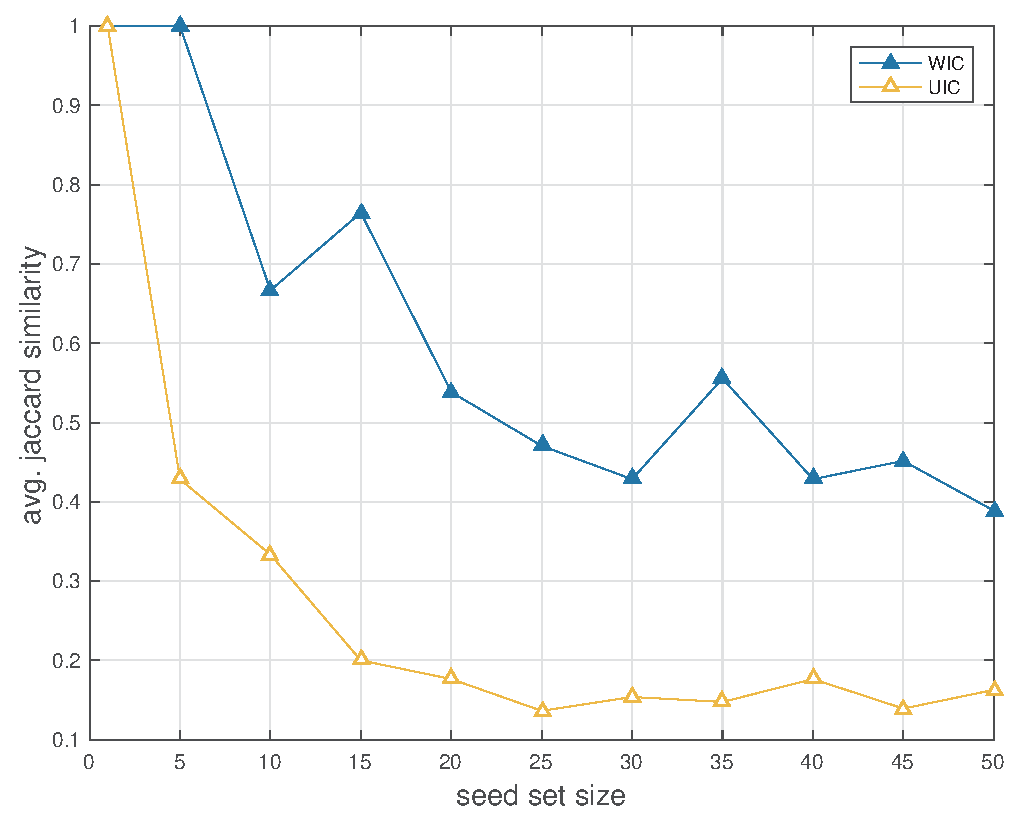
\includegraphics[width=\linewidth]{facebookJaccard}
     \caption{在\textit{Facebook}数据集上不同$k$下的Jaccard相似度对比}
     \label{fig:facebookJaccard}
   \end{minipage}
   \hfill
   \begin {minipage}{0.48\textwidth}
     \centering
     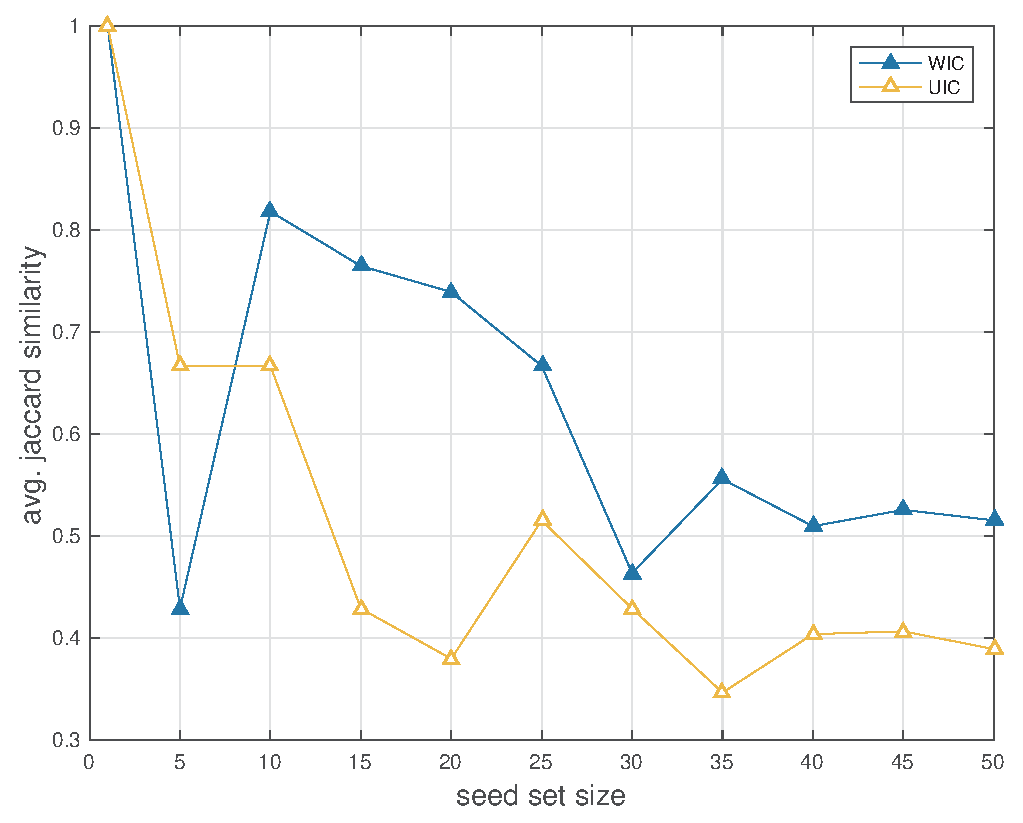
\includegraphics[width=\linewidth]{hepPhJaccard}
     \caption{在\textit{HepPh}数据集上不同$k$下的Jaccard相似度对比}
     \label{fig:hepPhJaccard}
   \end{minipage}
   \\
   \begin{minipage}{0.48\textwidth}
     \centering
     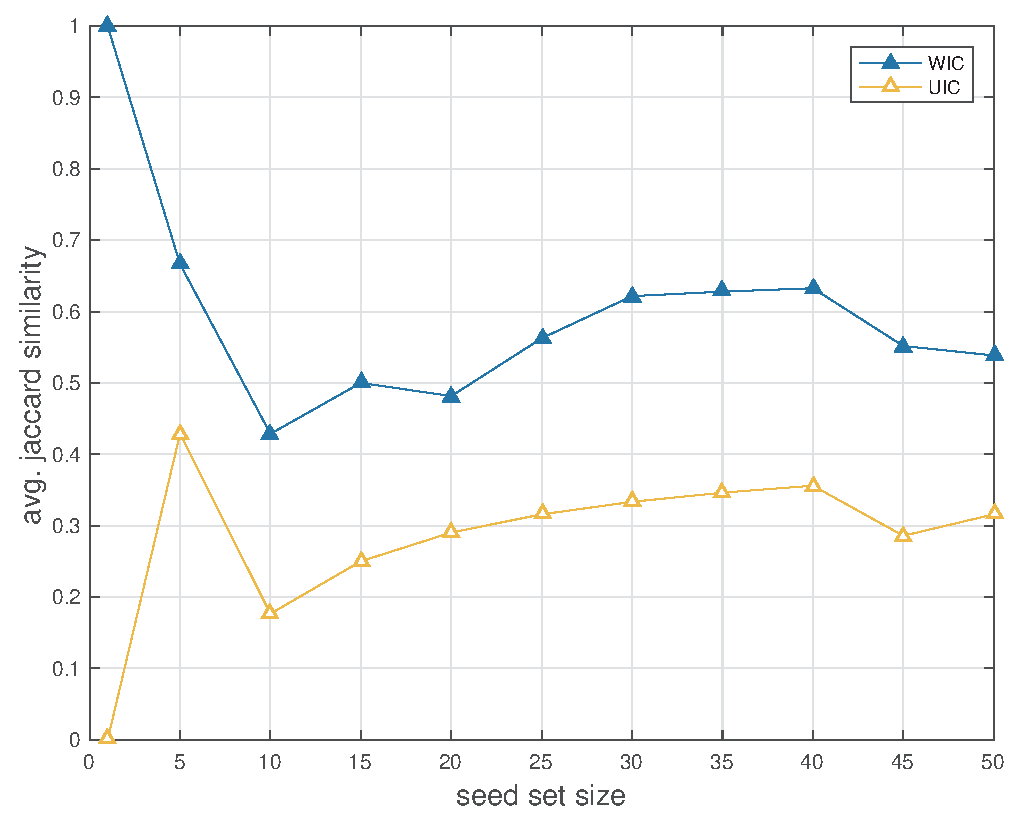
\includegraphics[width=\linewidth]{twitterJaccard}
     \caption{在\textit{Twitter}数据集上不同$k$下的Jaccard相似度对比}
     \label{fig:twitterJaccard}
   \end{minipage}
   \hfill
   \begin {minipage}{0.48\textwidth}
     \centering
     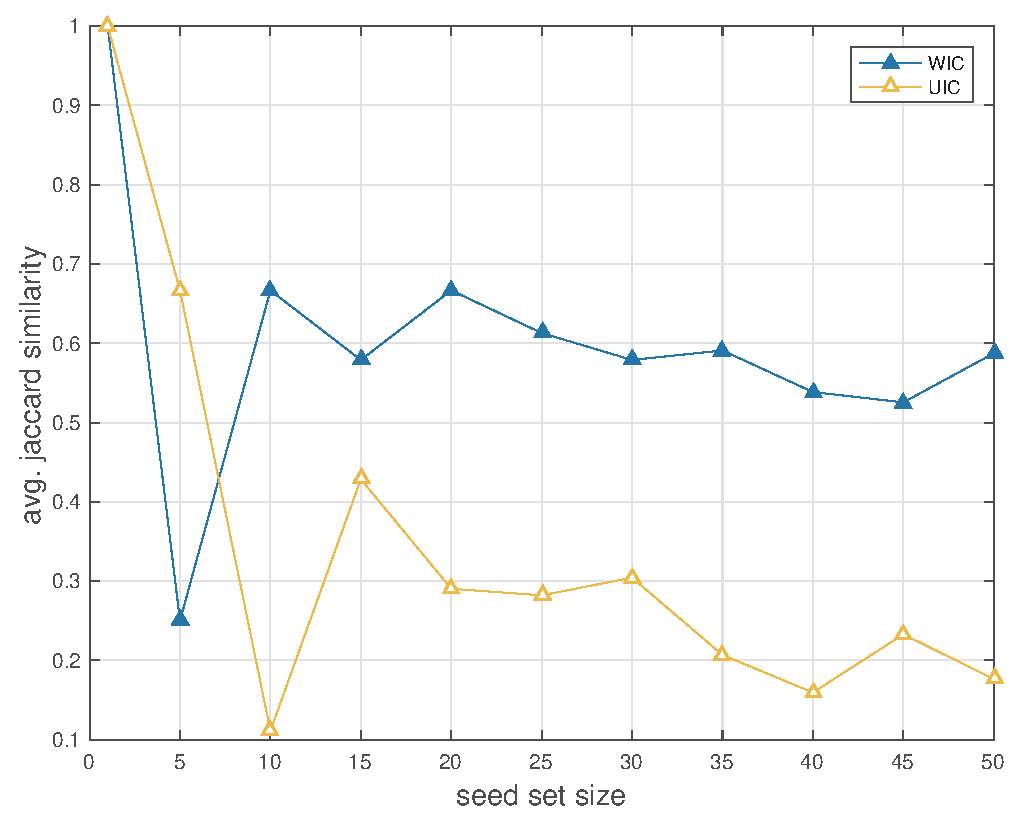
\includegraphics[width=\linewidth]{dblpJaccard}
     \caption{在\textit{DBLP}数据集上不同$k$下的Jaccard相似度对比}
     \label{fig:dblpJaccard}
   \end{minipage}
\end{figure}

第一组实验将反向效率采样算法与反向传播采样算法进行对比,来说明传播效率最大化问题与影响力最大化问题的区别。令反向效率采样算法求解最大化传播效率期望值得到的种子节点集合为$S$,反向传播采样算法求解最大化影响力期望值得到的种子节点集合为$S'$。我们可得到不同$k$下,集合$S$与集合$S'$之间的Jaccard相似度。令$J(S,S')$表示集合$S$与集合$S'$之间的Jaccard相似度,可形式化如下,
\begin{equation}\label{eq:jaccard}
    J(S,S') = \frac{\vert S \cap S' \vert}{\vert S \cup S' \vert}
\end{equation}
其中$\vert S \cap S' \vert$表示集合$S$与集合$S'$的交集大小,$\vert S \cup S' \vert$表示集合$S$与集合$S'$的并集大小。实验结果如图\ref{fig:facebookJaccard}至图\ref{fig:dblpJaccard}所示。从实验结果可知,在$k$较小的时候,例如$k=1$时,Jaccard相似度相似度是不稳定的。在$k=1$的情况下,\textit{Facebook}、\textit{HepPh}以及\textit{DBLP}网络中的$S=S'$,而\textit{Twitter}网络中的$S \neq S'$。由此可知,当$k$比较小的时候,使得网络有最大影响力期望值的节点也可能是使得网络有最大传播效率期望值的节点。当$k$比较小的时候,大部分节点处于未激活状态,能够激活尽可能多的节点也许就能获得更大的传播效率。随着$k$的增加,例如超过10以后,在均匀独立级联模型和加权独立级联模型下的$J(S,S')$值变得相对稳定。在均匀独立级联模型中$J(S,S')$约等于0.2,在加权独立级联模型中$J(S,S')$约等于0.5。因此,我们可知传播效率最大化问题的种子节点集合与影响力最大化问题的种子节点集合并不是相同的,即传播效率最大化问题与影响力最大化问题是两个不同的问题。

\subsection{算法精确度对比}
\label{subsec4:accuracy}
\begin{figure}[!ht]
   \begin{minipage}{0.48\textwidth}
     \centering
     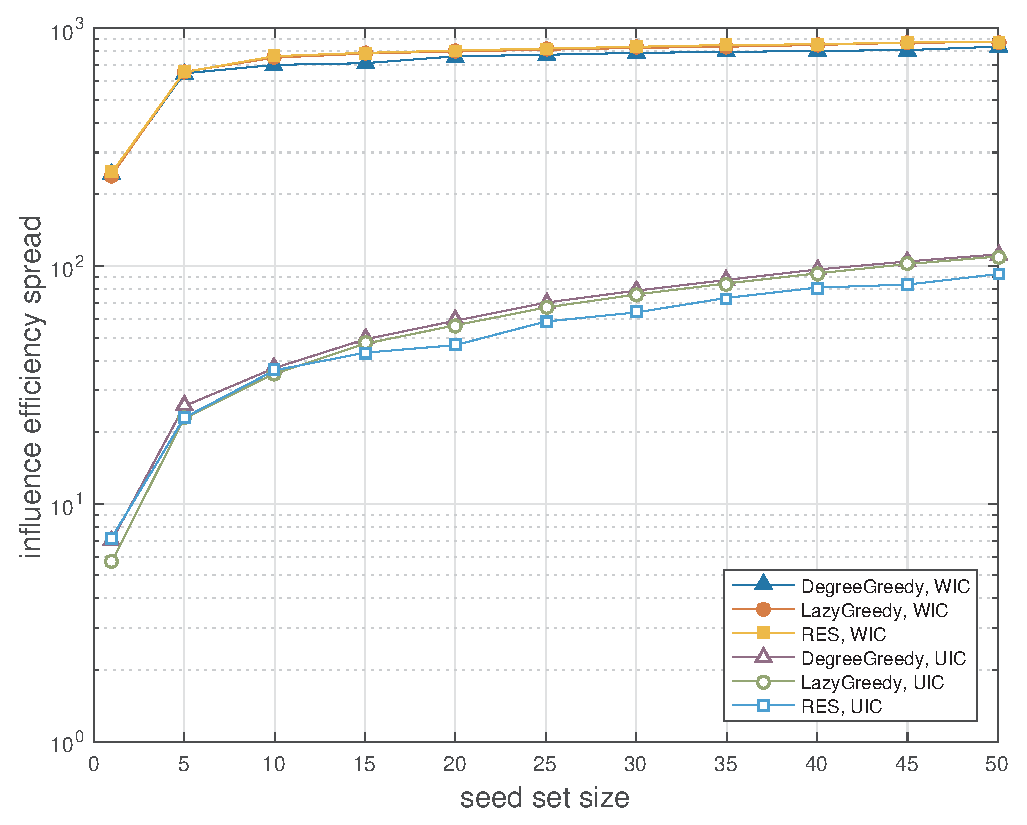
\includegraphics[width=\linewidth]{facebookEff}
     \caption{在\textit{Facebook}数据集上不同$k$下的传播效率对比}
     \label{fig:facebookEff}
   \end{minipage}
   \hfill
   \begin {minipage}{0.48\textwidth}
     \centering
     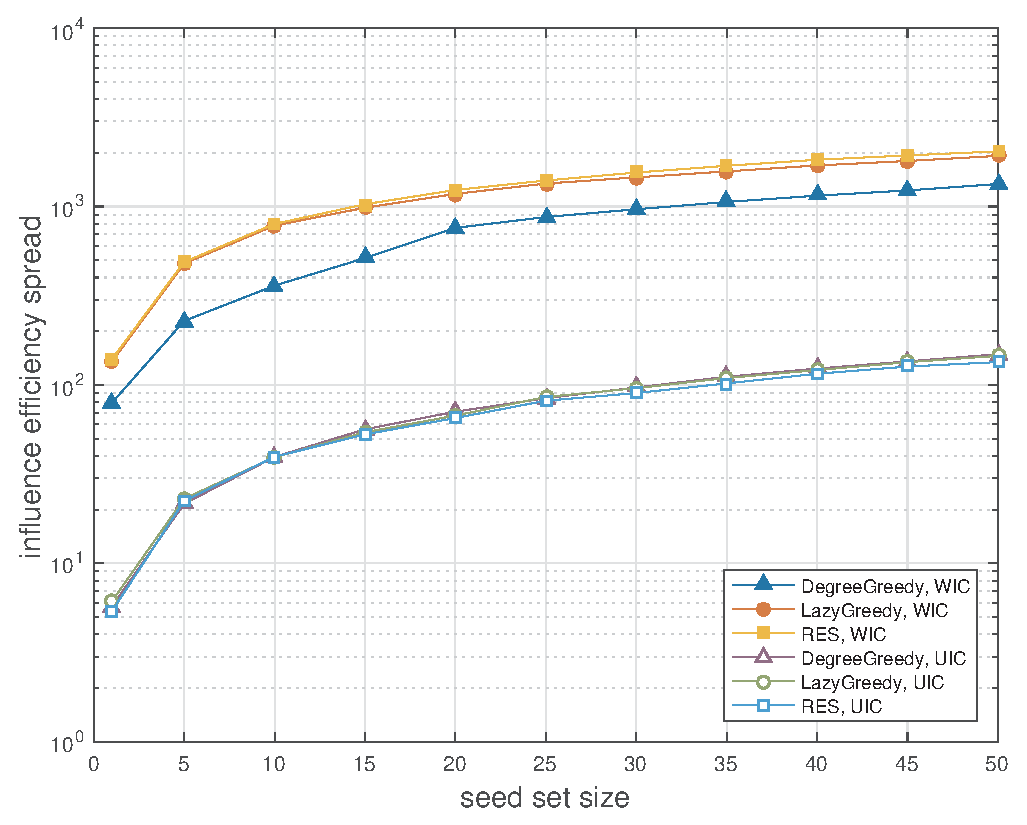
\includegraphics[width=\linewidth]{hepPhEff}
     \caption{在\textit{HepPh}数据集上不同$k$下的传播效率对比}
     \label{fig:hepPhEff}
   \end{minipage}
   \\
   \begin{minipage}{0.48\textwidth}
     \centering
     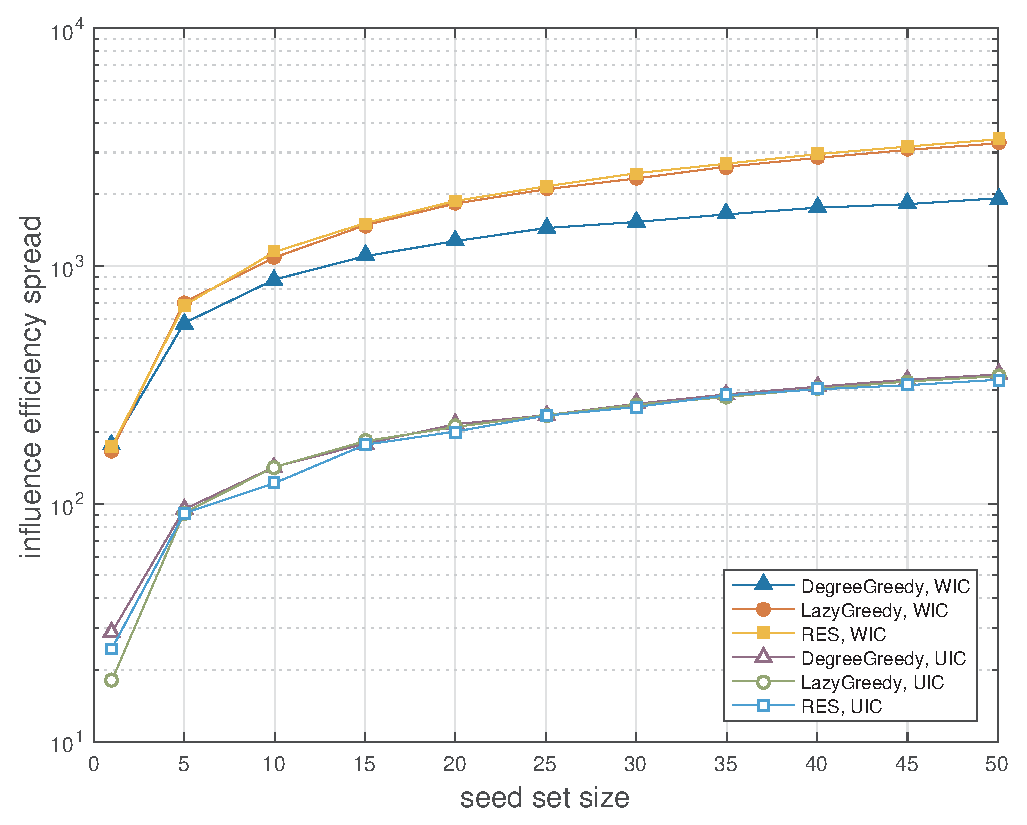
\includegraphics[width=\linewidth]{twitterEff}
     \caption{在\textit{Twitter}数据集上不同$k$下的传播效率对比}
     \label{fig:twitterEff}
   \end{minipage}
   \hfill
   \begin {minipage}{0.48\textwidth}
     \centering
     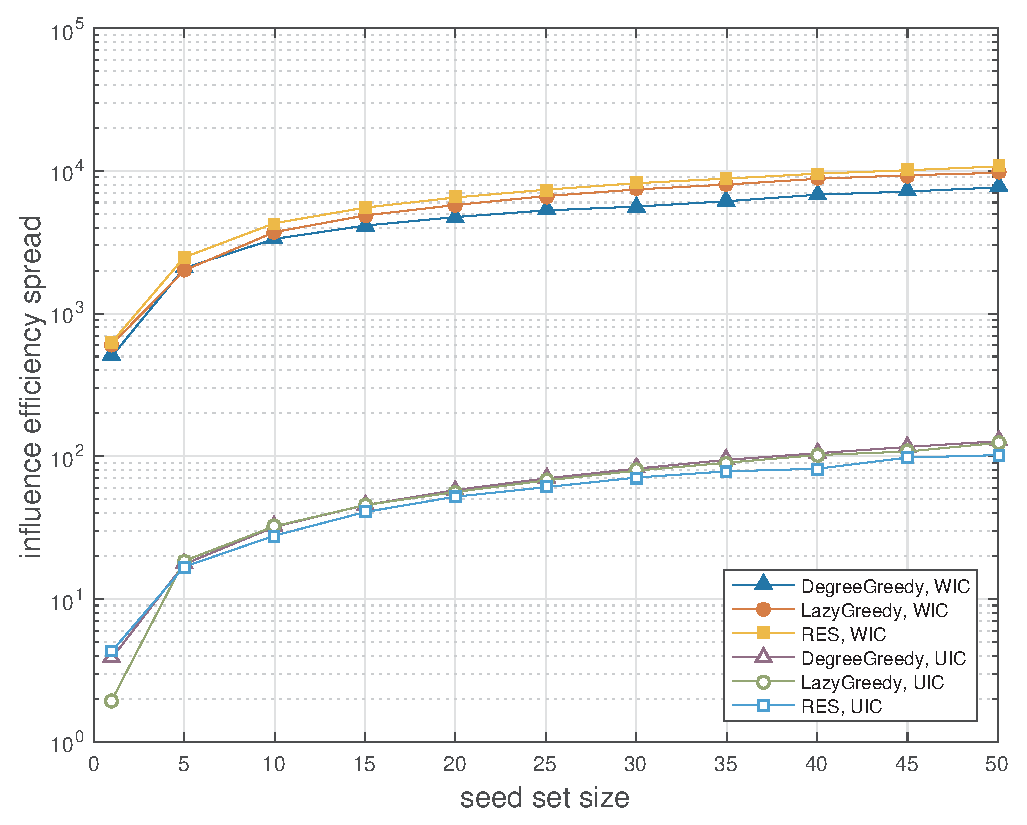
\includegraphics[width=\linewidth]{dblpEff}
     \caption{在\textit{DBLP}数据集上不同$k$下的传播效率对比}
     \label{fig:dblpEff}
   \end{minipage}
\end{figure}

在本小节中,我们计算各种算法得出种子节点集合的传播效率,对比各种算法的精确度。对于结果种子节点集合,我们运行10,000次蒙特卡罗模拟来估计信息传播过程中的传播效率。此外,对于每一个数据集,我们调整种子节点集合大小$k$从1到50来观察不同大小种子节点集合的传播效率。我们在均匀独立级联模型以及加权独立级联模型下进行实验,实验结果如图\ref{fig:facebookEff}至图\ref{fig:dblpEff}所示。如图所示,反向效率采样算法与惰性贪心算法、最大度算法在均匀独立级联模型下各数据集中的传播效率性能相似。这是由于在均匀独立级联模型下不能保证$\sum_{u \in \mathcal{V}}{p_{u,v}} = 1$的成立,且反向效率采样算法得到的近似最优解的近似率不高,所以在某些网络中(例如图\ref{fig:facebookEff}),反向效率采样算法的性能要稍差一些。但是我们可以得知,反向效率采样算法的精确度在最差的情况下(\textit{Facebook}网络)与最好结果相差少于17\%,不会相差一个数量级。在加权独立级联模型下,反向效率采样算法在各数据集中的精确度都是最高的,并且与惰性贪心算法的精确度相似,而最大度算法的精确度相比较低。例如在图\ref{fig:twitterEff}中$k=50$的情况下,最大度算法与反向效率采样算法的精确度相差56.5\%,即最大度算法得出种子节点集合的传播效率只有反向效率采样算法的一半左右。

由上述在均匀独立级联模型以及加权独立级联模型下各数据集上的实验结果可知,反向效率采样算法和惰性贪心算法都有理论上的精确度保证,性能优于启发式算法,例如最大度算法。

\subsection{运行时间对比}
\label{subsec4:runningTime}
\begin{figure}[!ht]
   \begin{minipage}{0.48\textwidth}
     \centering
     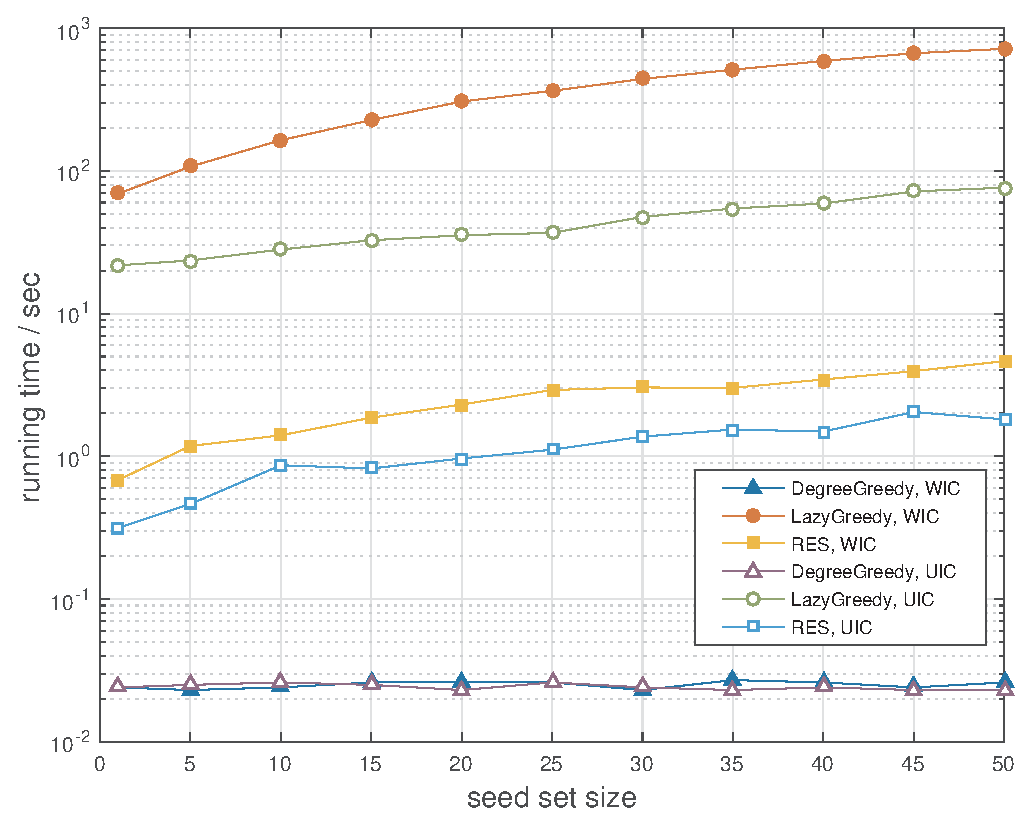
\includegraphics[width=\linewidth]{facebookTime}
     \caption{在\textit{Facebook}数据集上不同$k$下的运行时间对比}
     \label{fig:facebookTime}
   \end{minipage}
   \hfill
   \begin {minipage}{0.48\textwidth}
     \centering
     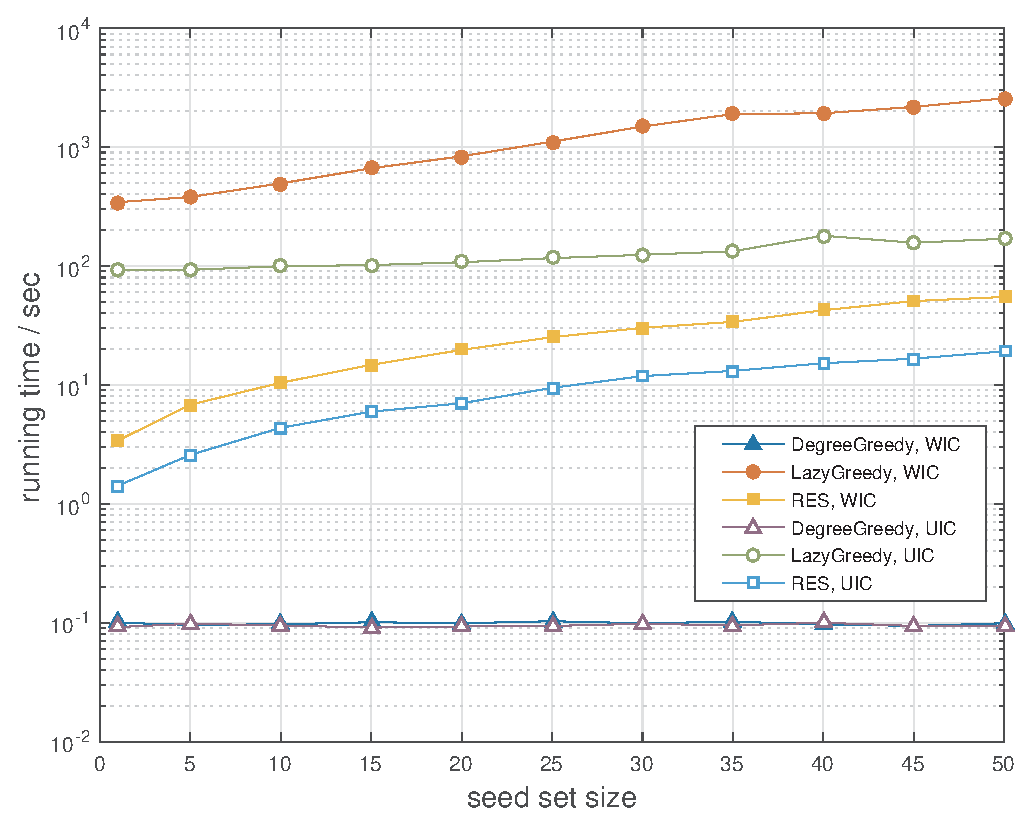
\includegraphics[width=\linewidth]{hepPhTime}
     \caption{在\textit{HepPh}数据集上不同$k$下的运行时间对比}
     \label{fig:hepPhTime}
   \end{minipage}
   \\
   \begin{minipage}{0.48\textwidth}
     \centering
     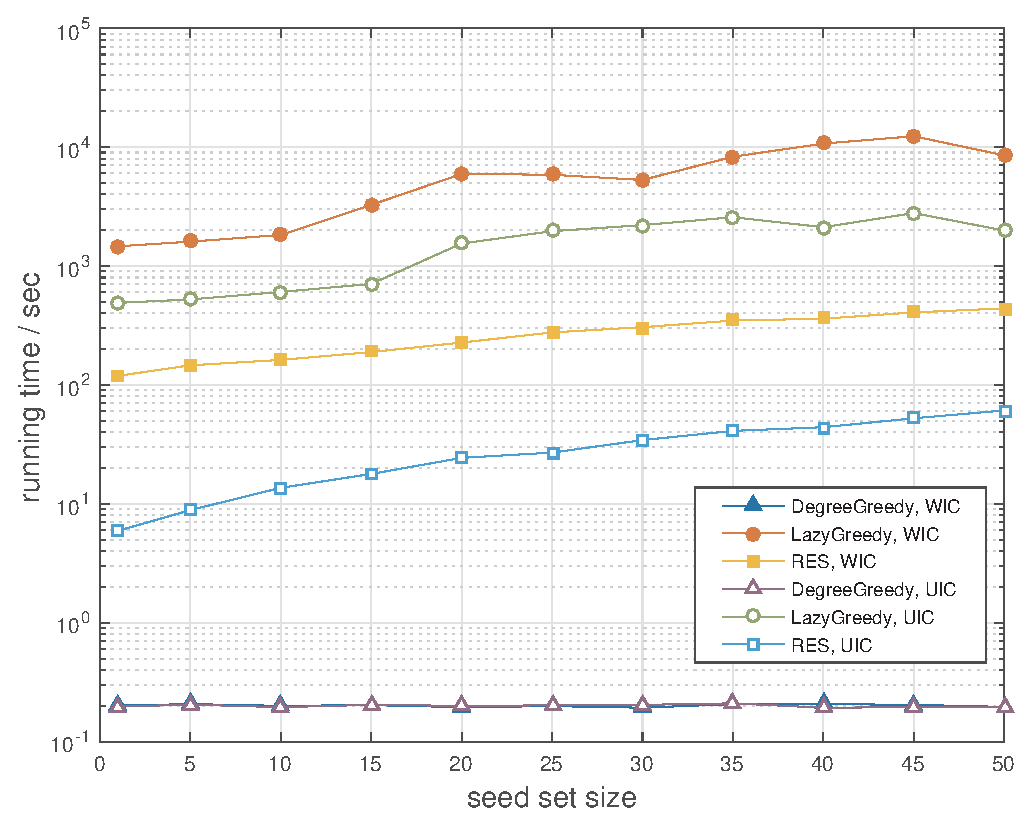
\includegraphics[width=\linewidth]{twitterTime}
     \caption{在\textit{Twitter}数据集上不同$k$下的运行时间对比}
     \label{fig:twitterTime}
   \end{minipage}
   \hfill
   \begin {minipage}{0.48\textwidth}
     \centering
     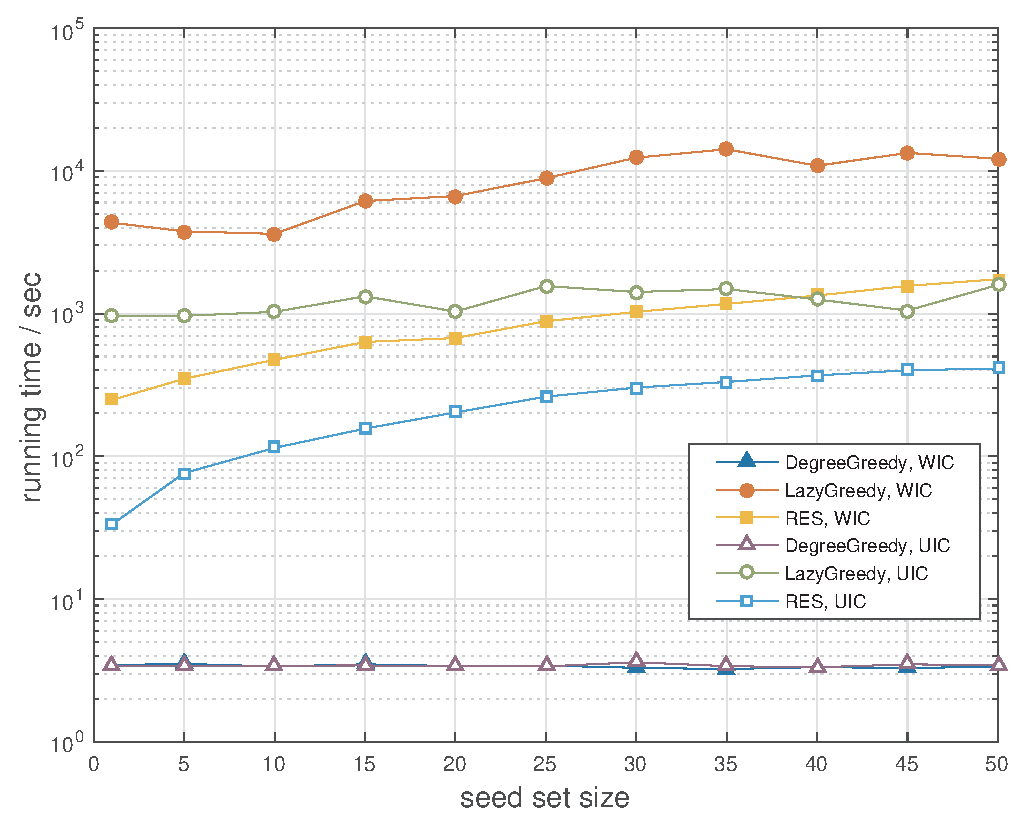
\includegraphics[width=\linewidth]{dblpTime}
     \caption{在\textit{DBLP}数据集上不同$k$下的运行时间对比}
     \label{fig:dblpTime}
   \end{minipage}
\end{figure}

本小节我们对各算法的运行时间进行对比实验。为了验证反向效率采样算法的效率,我们在均匀独立级联模型以及加权独立级联模型下各数据集上不同$k$的情况下,与惰性贪心算法以及最大度算法进行实验对比,结果如图\ref{fig:facebookTime}至图\ref{fig:dblpTime}。如图所示,在均匀独立级联模型以及加权独立级联模型下,反向效率采样算法相比惰性贪心算法都能提高一个数量级的效率。而最大度算法是一种启发式的算法,因此运行时间最少,且不随$k$的变化而变化,但是如第\ref{subsec4:accuracy}小节所示,该算法不能提供性能的保证。因为最大度算法算法简单,本小节利用该算法来作运行时间的一个下限基准。从图中我们可以得出,反向效率采样算法和惰性贪心算法的运行时间都随着$k$的增加而增加,其中惰性贪心算法运行时间的增长速率高于反向效率采样算法。例如,在图\ref{fig:twitterTime}中在$k=1$时,惰性贪心算法的运行时间约为反向效率采样的10倍,在$k=50$时,增长为约20倍。因此,反向效率采样算法的效率优于其他的算法。

\subsection{可扩展性}
\label{subsec4:scalability}
\begin{figure}[ht]
    \centering
    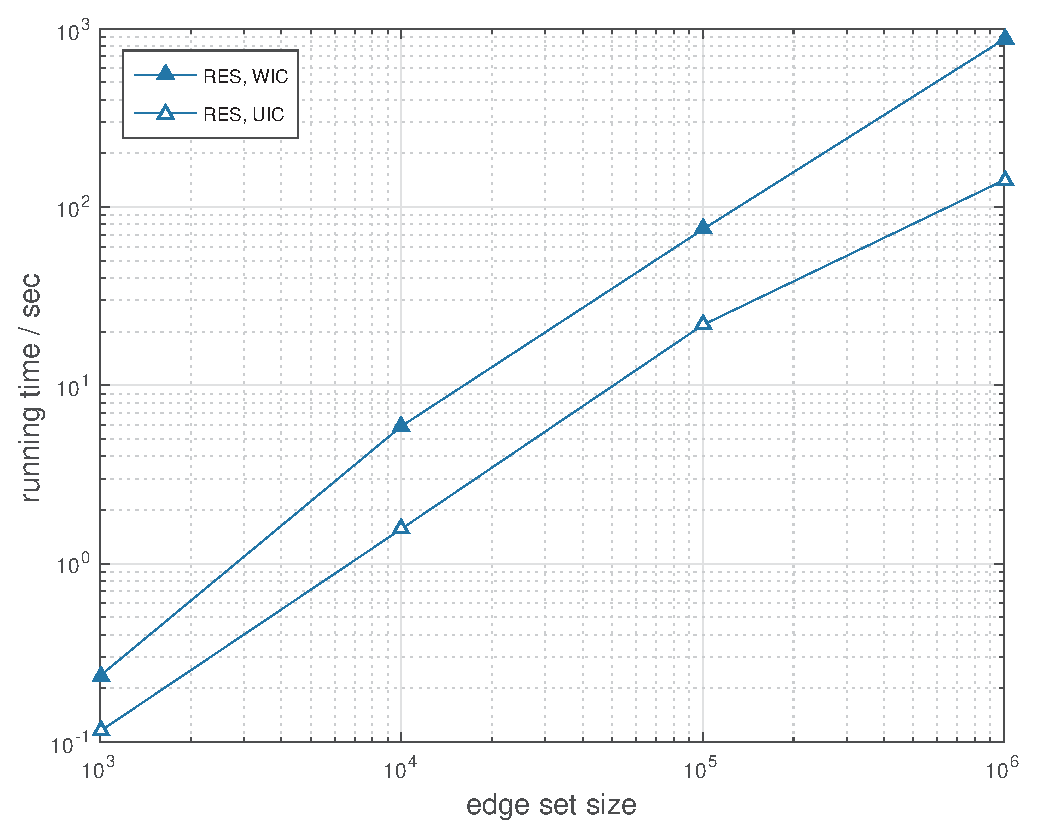
\includegraphics[width=0.5\textwidth]{resScalability}
    \caption{反向效率采样算法的可扩展性}
    \label{fig:scalability}
\end{figure}

本小节进行了反向效率采样算法的可扩展性实验。实验使用\textit{DBLP}网络来生成各种大小的子图。生成过程如下所示。首先,我们随机地选取图中的一个节点,然后做宽度优先搜索来添加边到子图中,该过程直到子图的大小满足要求时停止。如果宽度优先搜索过程在子图大小没有满足前就停止了,那么在重新随机地选择一个不在目前子图中的节点,继续进行宽度优先搜索,重复上述过程直到满足要求。利用该方法,我们可以得到各种大小的子图。本小节的实验中,我们令子图的边的大小从$m=1,000$到$m=1,000,000$变化,然后运行反向效率采样算法,记录运行的时间。在均匀独立级联模型以及加权独立级联模型下的实验结果如图\ref{fig:scalability}所示。由图可知,随着图大小的增长,运行时间的增长是线性的。因此,反向效率采样算法是可扩展的。
\section{本章小结}
\label{sec4:conclusion}
为了更好地理解网络中的传播效率,本章将信息传播过程中的传播时延考虑在内,提出了一个新的问题,传播效率最大化问题。该问题的目的在于最大化网络中的传播效率期望值。然后,我们证明了在独立级联模型下,传播效率最大化问题是一个NP-难的问题,而且计算传播效率的过程是一个\#P-难的问题。为了解决该问题,我们证明了在独立级联模型下,传播效率函数的期望值是单调且子模性的。基于上述的性质,我们设计了三种算法来解决该问题。最后,我们在真实的数据集上进行了一系列的实验来验证所提出的算法。实验结果表明了传播效率最大化问题与影响力最大化问题的不同,证明了提出的算法的正确性和有效性。本章所研究的内容对充分理解信息传播过程有着一定的帮助。

